\documentclass[journal]{IEEEtran}

\usepackage{graphicx}
\usepackage{booktabs}
\usepackage{amsmath,amssymb}
\usepackage{multirow}
\usepackage{array}
\usepackage{xcolor}
\usepackage{tikz}
\usetikzlibrary{shapes.geometric,arrows.meta,positioning,fit,backgrounds,calc}
\usepackage[colorlinks=true,linkcolor=black,citecolor=black,urlcolor=blue]{hyperref}
\usepackage{url}
\usepackage{siunitx}
\sisetup{detect-weight=true,detect-family=true}
\DeclareSIUnit{\lufs}{LUFS}
\DeclareSIUnit{\point}{point}
\DeclareSIUnit{\sample}{sample}

\newcommand{\ttf}[1]{\texttt{\footnotesize #1}}

% flowchart styles
\tikzset{
  blk/.style   = {draw, rounded corners=1.6pt, align=center, inner sep=3pt,
                  font=\scriptsize, line width=0.5pt},
  data/.style  = {blk, fill=black!4},
  proc/.style  = {blk, fill=cyan!10,   draw=cyan!55!black},
  null/.style  = {blk, fill=yellow!25, draw=black!60, densely dashed},
  sumbox/.style= {blk, fill=black!8, line width=0.8pt},
  ar/.style    = {-{Stealth[length=4pt]}, line width=0.5pt},
  lbl/.style   = {font=\tiny\itshape, inner sep=1pt}
}

\begin{document}

\title{What the Model Learns from Coded Audio:\\
Null-Calibrated Feature Attribution in\\
Explainable Speech Emotion Recognition}

\author{Akshath~R%
\thanks{Manuscript prepared \today.}%
\thanks{A.~R is an independent researcher (e-mail: akshath.r333@gmail.com).}%
\thanks{Code, stimulus manifests, the feature table schema, and every result
file underlying the tables and figures are released with this paper; see the
Data Availability Statement.}}

\markboth{IEEE Transactions on Affective Computing}%
{R: Null-Calibrated Feature Attribution Under Perceptual Audio Coding}

\maketitle

\begin{abstract}
Speech emotion recognition is validated on uncompressed audio and deployed on
coded audio. Whether that gap matters has been asked of accuracy; we ask it of
the evidence, using models whose evidence can be read exactly. Fifteen
classifiers and a small neural network are fitted to 436 \emph{named} acoustic
descriptors over CREMA-D, rendered in four conditions from one canonical
reference: uncompressed WAV, MP3 and MP4/AAC at
\SI{64}{\kilo\bit\per\second}, and an AAC re-wrap that holds the codec output
fixed while changing the container. Three results follow. First, the
catastrophic cross-format collapse is train/serve mismatch and nothing else: a
kernel machine trained on WAV scores 0.203 balanced accuracy on MP3, but the
same model \emph{trained} on MP3 scores 0.589 against 0.586 on clean audio, so
the affective information survives the codec intact. Second, what the model
learns from that information does change, and the change is legible because the
features are named: an entropy tree fitted per condition selects the same root
descriptor (\ttf{prosody\_intensity\_std}) in all four conditions with
information gain stable to 0.003 bits, but AAC displaces the threshold by
1.3\,\% and replaces the depth-1 descriptor, while the MP3 tree does not.
Third --- and this is the methodological contribution --- a codec effect on a
feature-importance ranking is uninterpretable without a null, because the
ranking is fragile. Refitting on identical audio with different tie-breaking
retains 24.2 of 25 top features, but an \emph{informationally empty} container
re-wrap already costs 8.4 of them. Against that floor the codec effects are real
but far smaller than they look: MP3 retains 12.6 and AAC 10.7
($p\leq1.1\times10^{-3}$, paired within resampled training sets), so roughly
three fifths of the apparent displacement is generic perturbation sensitivity,
not codec-specific. We report the complete 436-column inventory and the full
per-condition split structure, and argue that attribution-shift claims in
affective computing require a matched empty-perturbation control as standard.
\end{abstract}

\begin{IEEEkeywords}
Speech emotion recognition, explainable artificial intelligence, perceptual
audio coding, feature attribution, decision trees, information gain, covariate
shift, null calibration, affective computing.
\end{IEEEkeywords}

\section{Introduction}
\IEEEPARstart{A}{udio} almost never reaches an inference endpoint in the
representation in which it was captured. Contact-centre archives hold MP3;
streaming clients negotiate Opus or AAC; broadcast pipelines resample and
requantise. Evaluation practice runs the other way: benchmarks are distributed
as uncompressed WAV and read directly from disk.

The gap is usually dismissed on a reasonable argument. Any ingestion path
decodes to linear PCM before feature extraction, so the delivery format is an
implementation detail. Where the argument has been tested, it has been tested on
accuracy, and the answers are mixed: Reddy and
Vijayarajan~\cite{reddy2020compression} report codec effects on speech emotion
recognition (SER) that are real, modest, and dependent on the front end.

Accuracy is the wrong instrument for a system that is increasingly required to
say not only \emph{what} it concluded but \emph{why}. A deployed affective
system may surface an attribution over acoustic evidence to a clinician, an
auditor, or a quality-assurance analyst. That second output has its own
robustness properties, and they are not implied by the first. Ghorbani et
al.~\cite{ghorbani2019fragile} established for image classifiers that
perceptually indistinguishable inputs receiving identical predictions can be
assigned materially different attributions; Alvarez-Melis and
Jaakkola~\cite{alvarez2018robustness} showed the same fragility more generally.
Both used adversarially constructed perturbations. A transcode is not
adversarial. It is routine, ubiquitous, and nobody logs it.

\subsection{Why interpretable models, and why named features}
Answering an evidential question requires a model whose evidence can be
inspected, and inspectability is not one property. An end-to-end audio model
learns its own representation, so an attribution over one of its latent
dimensions is not a claim about anything an acoustician would recognise. A model
fitted to \emph{named} descriptors in the GeMAPS~\cite{eyben2016gemaps} and
openSMILE~\cite{eyben2010opensmile} tradition is different: an attribution over
\ttf{prosody\_cpps} is a claim about breathiness, and a decision-tree split on
\ttf{spectral\_contrast\_6\_mean} is a claim about the \SIrange{6}{8}{\kilo\hertz}
band. This paper is confined to that regime deliberately. Everything reported
here is exact rather than estimated, checkable against an acoustic reading, and
reproducible from the released artefacts.

\subsection{The problem with attribution-shift claims}
A claim of the form ``compression changed which features the model relies on''
is easy to produce and hard to justify. Feature-importance rankings are
notoriously unstable: two descriptors that split almost equally well can swap,
and one swap near a tree's root reroutes every descendant. A ranking can
therefore move a long way without the data having moved at all. The literature
already contains the general warning --- Adebayo et al.~\cite{adebayo2018sanity}
show that some saliency methods are independent of the model they claim to
explain, and Krishna et al.~\cite{krishna2022disagreement} show that different
methods disagree on the same fitted model --- but the specific discipline it
implies, measuring the shift induced by a manipulation that carries no
information, is not standard practice.

We adopt it here, and it changes the answer. Our design supplies a natural empty
perturbation: the same codec output routed through two containers. Once that
floor is measured, most of the apparent codec effect on importance rankings
turns out to be generic sensitivity to any input perturbation.

\subsection{Contributions}
\begin{enumerate}
\item \textbf{A matched-format decomposition of the codec effect.} Training and
      serving in the same coded condition recovers essentially all of a
      catastrophic cross-format loss --- up to 38.6 balanced-accuracy points ---
      establishing that \SI{64}{\kilo\bit\per\second} coding does not remove the
      affective information, it moves it out of the range the model was fitted
      on (Section~\ref{sec:matched}).
\item \textbf{Per-condition tree structure as a readable attribution.} An
      entropy tree fitted independently on each condition exposes exactly which
      test the codec changes and which it leaves alone, at the level of a named
      descriptor and a numeric threshold (Section~\ref{sec:trees}).
\item \textbf{Null calibration for feature-importance shift.} Three floors ---
      estimator tie-breaking, actor resampling, and an informationally empty
      container re-wrap --- with a paired within-sample design that separates the
      codec effect from all three (Section~\ref{sec:null}).
\item \textbf{A diagnosable and cheap repair.} Neutralising a single named
      descriptor recovers 98\,\% of a kernel machine's loss and 92\,\% of a
      network's, at no cost on uncompressed audio
      (Section~\ref{sec:neutralise}).
\item \textbf{Two negative results retained rather than smoothed.} Post-hoc
      attribution methods disagree substantially on the same fitted model, and a
      global attribution ranking can report ``nothing changed'' while the
      classifier has stopped working (Sections~\ref{sec:methods-disagree},
      \ref{sec:blindspot}).
\item \textbf{A complete, released inventory.} All 436 descriptors are defined
      and enumerated (Appendix~\ref{app:features}), and every internal node of
      every per-condition tree is tabulated (Appendix~\ref{app:splits}).
\end{enumerate}

\section{Related Work}

\subsection{Perceptual coding and speech task degradation}
Degradation of speech systems under lossy coding is documented but shallowly
characterised. Reddy and Vijayarajan~\cite{reddy2020compression} find that
standard codecs reduce SER accuracy with a magnitude conditional on both codec
family and feature representation, which already implies that coding interacts
with the front end rather than degrading performance uniformly.

Of greater methodological consequence is a result from neural codec
benchmarking. Wu et al.~\cite{wu2024codecsuperb} demonstrate that signal-domain
fidelity metrics \emph{fail to predict} the retention of task-relevant
information: a codec can score well under reconstruction error while discarding
paralinguistic content that downstream tasks require. We take this seriously
enough to report signal-domain displacement and model behaviour as separate
quantities throughout, treating neither as a surrogate for the other.

\subsection{Interpretability for tabular and audio models}
Post-hoc attribution has converged on a small set of workhorses: local surrogate
fitting~\cite{ribeiro2016lime}, Shapley-value
attribution~\cite{lundberg2017shap} with an exact polynomial-time algorithm for
tree ensembles~\cite{lundberg2020treeshap}, and permutation importance. For
differentiable models, path-integral methods~\cite{sundararajan2017ig} and
reference-based decompositions~\cite{shrikumar2017deeplift} are standard, and
are available in consolidated form~\cite{kokhlikyan2020captum}. Broad surveys
map the space~\cite{guidotti2018survey}; Rudin~\cite{rudin2019stop} argues that
for high-stakes decisions the post-hoc layer should be replaced by an
intrinsically interpretable model, a position our
Section~\ref{sec:leaderboard} result speaks to directly and unfavourably.

Transfer of these methods to audio is contested. Haunschmid et
al.~\cite{haunschmid2020audiolime} argue that audio explanations should satisfy
a \emph{listenability} criterion and that transplanting image-segmentation logic
onto time--frequency representations yields components with no perceptual
correlate. Related formulations appear in~\cite{becker2018audiomnist}
and~\cite{sotirou2024musiclime}, and Nasr et al.~\cite{nasr2025beyond} extend
the critique to speech emotion specifically, observing that a salient
time--frequency region is not thereby an acoustically meaningful one. Attributing
over named acoustic descriptors sidesteps this objection rather than answering
it: every unit of attribution here has a phonetic reading by construction, at
the cost of confining the model to hand-designed features.

\subsection{Attribution stability as a validity requirement}
The literature most directly load-bearing for this paper concerns the fragility
of attribution itself. Ghorbani et al.~\cite{ghorbani2019fragile} show that
attributions can be substantially altered by perturbations below the threshold
of perception while predictions and confidences remain stable. Adebayo et
al.~\cite{adebayo2018sanity} demonstrate that certain widely deployed saliency
methods are statistically independent of both model parameters and
data-generating process, producing outputs with the surface form of explanation
and none of its content. Krishna et al.~\cite{krishna2022disagreement} document
that different explanation methods routinely disagree on the same model, and
that practitioners resolve the disagreement by unprincipled means.

The joint implication is that attribution stability must be \emph{measured
against a null}, not presumed. Section~\ref{sec:null} operationalises that
requirement for the specific object at issue here, a feature-importance ranking,
and finds that the requirement is not a formality: it changes the size of the
reported effect by a factor of roughly two and a half.

\subsection{Distribution shift}
The mechanism we identify is textbook covariate
shift~\cite{morenotorres2012shift}, with one unusual property. The shifted
variable is not a proxy for anything the label depends on --- masking it costs
nothing on clean audio (Section~\ref{sec:neutralise}) --- so the shift is pure
contamination rather than a change in the predictive relationship. That is what
makes the repair as cheap as it turns out to be.

\subsection{Where the gap lies}
Coding effects are characterised for accuracy but not for evidence. Attribution
fragility is characterised for vision under adversarial perturbation but not for
audio under ecologically routine degradation. We identify no prior work that
isolates the container under a verified signal-invariance constraint, and none
that calibrates a feature-importance shift against a matched empty perturbation.

\section{Corpus, Stimuli, and Conditions}\label{sec:design}

\begin{figure*}[!t]
\centering
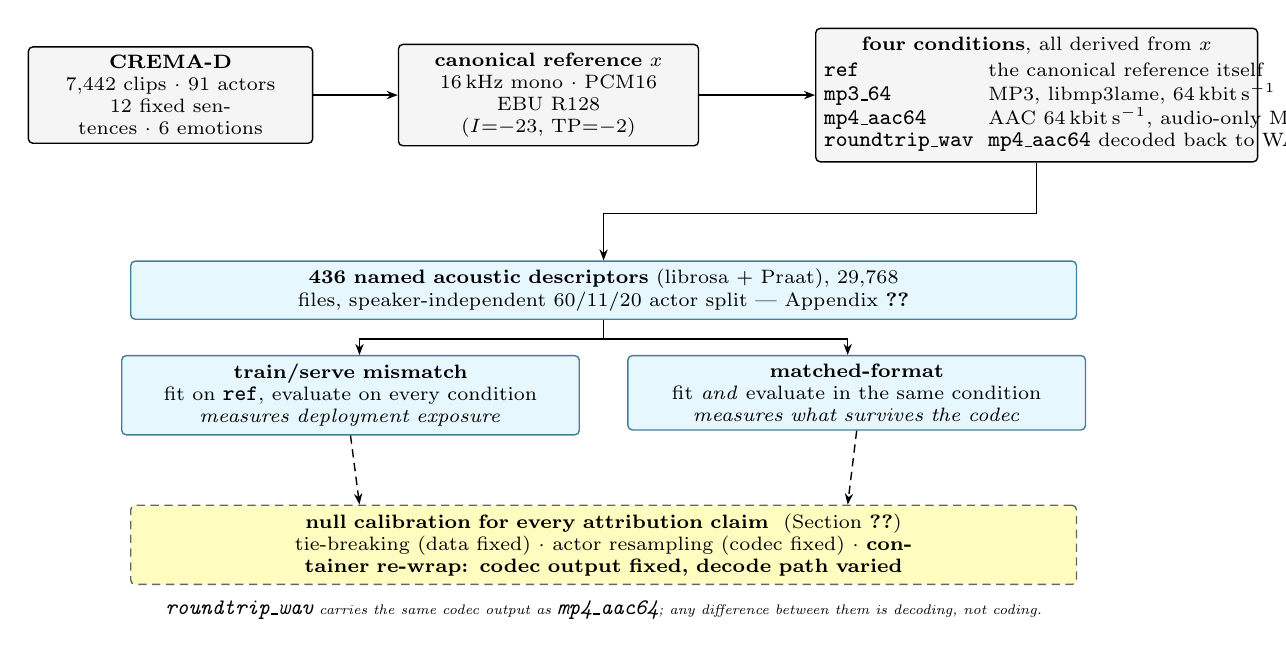
\begin{tikzpicture}[x=1mm, y=1mm]
\node[data, text width=34mm] (corpus) at (0,0)
  {\textbf{CREMA-D}\\7{,}442 clips $\cdot$ 91 actors\\
   12 fixed sentences $\cdot$ 6 emotions};
\node[data, text width=36mm] (ref) at (48,0)
  {\textbf{canonical reference} $x$\\
   \SI{16}{\kilo\hertz} mono $\cdot$ PCM16\\
   EBU R128 ($I{=}{-}23$, TP${=}{-}2$)};
\node[data, text width=54mm] (cond) at (110,0)
  {\textbf{four conditions}, all derived from $x$\\[1.5pt]
   \begin{tabular}{@{}l@{\ \ }l@{}}
   \ttf{ref}           & the canonical reference itself\\
   \ttf{mp3\_64}       & MP3, libmp3lame, \SI{64}{\kilo\bit\per\second}\\
   \ttf{mp4\_aac64}    & AAC \SI{64}{\kilo\bit\per\second}, audio-only MP4\\
   \ttf{roundtrip\_wav}& \ttf{mp4\_aac64} decoded back to WAV\\
   \end{tabular}};
\draw[ar] (corpus) -- (ref);
\draw[ar] (ref) -- (cond);

\draw[line width=0.5pt] (cond.south) -- (110,-15) -- (55,-15);
\draw[ar] (55,-15) -- (55,-21);

\node[proc, text width=118mm, anchor=north] (feat) at (55,-21)
  {\textbf{436 named acoustic descriptors} (librosa $+$ Praat), 29{,}768 files,
   speaker-independent 60/11/20 actor split --- Appendix~\ref{app:features}};

\node[proc, text width=56mm, anchor=north east] (mis) at (52,-33)
  {\textbf{train/serve mismatch}\\
   fit on \ttf{ref}, evaluate on every condition\\
   \emph{measures deployment exposure}};
\node[proc, text width=56mm, anchor=north west] (mat) at (58,-33)
  {\textbf{matched-format}\\
   fit \emph{and} evaluate in the same condition\\
   \emph{measures what survives the codec}};
\draw[ar] (feat.south) -- (55,-31) -- (24,-31) -- (24,-33);
\draw[ar] (55,-31) -- (86,-31) -- (86,-33);

\node[null, text width=118mm, anchor=north] (null) at (55,-52)
  {\textbf{null calibration for every attribution claim}\ \ (Section~\ref{sec:null})\\
   tie-breaking (data fixed) $\cdot$ actor resampling (codec fixed) $\cdot$
   \textbf{container re-wrap: codec output fixed, decode path varied}};
\draw[ar, densely dashed] (mis.south) -- (24,-52);
\draw[ar, densely dashed] (mat.south) -- (86,-52);

\node[lbl, anchor=north, below=1.6mm of null]
  {\ttf{roundtrip\_wav} carries the same codec output as \ttf{mp4\_aac64};
   any difference between them is decoding, not coding.};
\end{tikzpicture}
\caption{The design. Every condition descends from a single canonical reference
$x$, so no format contrast can be confounded by a divergent resampling or gain
path. The same models are fitted twice --- once on uncompressed audio and served
compressed, once trained and served in the same condition --- and the difference
between those two readings is the paper's first result. Every attribution claim
is evaluated against a floor measured on a manipulation that carries no coding
information.}
\label{fig:framework}
\end{figure*}

\subsection{Corpus}
CREMA-D~\cite{cao2014cremad} comprises 7{,}442 clips from 91 actors, each
delivering one of twelve fixed sentences in one of six acted emotions (anger,
disgust, fear, happiness, neutral, sadness), with crowd ratings collected
separately for voice-only, face-only and audio-visual presentation.

The fixed lexical inventory is methodologically load-bearing. Holding the words
constant across emotions and conditions removes the lexical channel as a source
of discriminative variance, so any recovered signal must be carried by acoustic
realisation --- which is precisely what perceptual coding operates on.

For reference throughout: CREMA-D's own crowd raters, hearing audio alone,
matched the actor's intended emotion on only 45.5\,\% of clips, with per-class
recall ranging from 0.966 (neutral) to 0.164 (sad). Models trained on the
\emph{intended} label can exceed this because they exploit systematic acting
cues human listeners do not consciously decode; the figure is reported as
context for absolute accuracy, not as a target.

\subsection{Reference construction and conditions}
The canonical reference is \SI{16}{\kilo\hertz} monophonic 16-bit linear PCM,
loudness-normalised to EBU~R128 ($I=\SI{-23}{\lufs}$, LRA${}=7$,
TP${}=\SI{-2}{\decibel}$). Coded conditions are produced from that reference by a
single encoder invocation each, and all decoding passes through one identical
FFmpeg call so that the decoder never confounds the codec.

The fourth condition is the identification device. \ttf{roundtrip\_wav} is the
AAC bitstream of \ttf{mp4\_aac64} decoded and re-wrapped as WAV: the same codec
output, a different container and one additional int16 quantisation. It is not
bit-identical to the direct MP4 decode --- the WAV path requantises --- but its
median standardised feature difference is $|\mathrm{SMD}|=7.6\times10^{-5}$,
with only 12 of 436 descriptors exceeding $0.05$. That is the noise floor of
this study, and Section~\ref{sec:null} uses it as an informationally empty
perturbation rather than merely reporting it as small.

Extraction over $7{,}442\times4=29{,}768$ files failed on exactly one clip in
all four conditions, \ttf{1076\_MTI\_SAD\_XX}, which the corpus documentation
lists as having no audio. The remaining 7{,}441 clips form the analysis set.

\subsection{What the codec does to the descriptors}\label{sec:signal}
Fig.~\ref{fig:signal} characterises the manipulation before any model is
involved. Two mechanisms are distinguishable and they behave differently.

\begin{figure*}[!t]
\centering
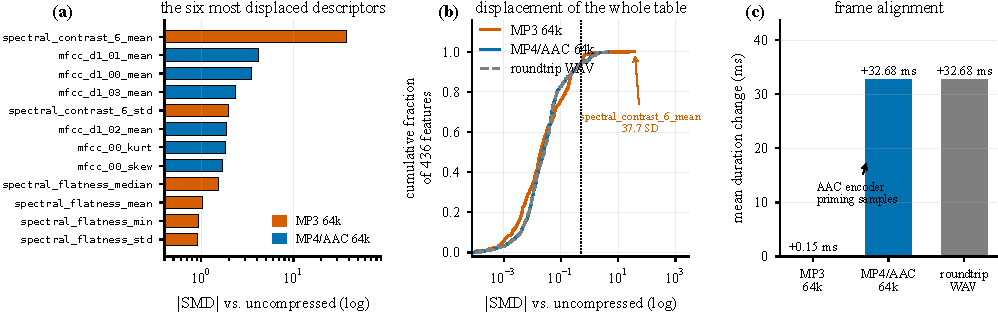
\includegraphics[width=\textwidth]{figs/fig_signal.pdf}
\caption{The coding manipulation, measured on the feature table over 7{,}441
clips. (a)~The six most displaced descriptors under each codec. MP3's
displacement is concentrated: \ttf{spectral\_contrast\_6\_mean}, which summarises
the \SIrange{6}{8}{\kilo\hertz} band, moves by 37.7 pooled standard deviations.
AAC's is diffuse and lands on delta-MFCC means, the frame-aligned temporal
derivatives. (b)~Empirical CDF of the absolute standardised mean difference of
all 436 descriptors. The median shift is negligible ($\approx0.02$); the tail is
not. (c)~AAC inserts encoder priming samples, lengthening every clip by
\SI{32.68}{\milli\second}; MP3 adds \SI{0.15}{\milli\second}.}
\label{fig:signal}
\end{figure*}

\textbf{MP3 abandons the top octave.} Perceptual bit allocation quantises the
highest band coarsely and zeroes masked bins, so
\ttf{spectral\_contrast\_6\_mean} moves from 16.38 to 46.54 and spectral flatness
collapses in parallel (mean $0.0189\rightarrow0.0066$) because the residual
spectrum is far less noise-like. Measured in \emph{training-set} standard
deviations the shift is $38.6\sigma$: the descriptor arrives at inference time in
a range no model fitted on clean audio has ever seen.

\textbf{AAC shifts frame alignment.} Encoder priming lengthens every clip by
\SI{32.68}{\milli\second}, uniformly, which perturbs every frame-aligned
temporal derivative a little rather than destroying one band. The largest AAC
shifts are consequently all delta-MFCC means (\ttf{mfcc\_d1\_01\_mean},
$\mathrm{SMD}=-4.16$). We flag a caveat here rather than in the limitations,
because it bears on how the number should be read: delta means sit near zero
with small standard deviations, so their standardised shifts are inflated
relative to their absolute change. The duration measurement is the harder
evidence for the padding mechanism.

\section{Feature Representation}\label{sec:features}

Each file is reduced to 436 named descriptors in four families, every
frame-level contour collapsed to eight order statistics (mean, standard
deviation, minimum, maximum, median, interquartile range, skewness, excess
kurtosis). Appendix~\ref{app:features} defines every descriptor and enumerates
every column; the summary is:

\begin{itemize}
\item \textbf{spectral} (114): centroid, bandwidth, roll-off (85/95\,\%),
flatness, flux, entropy, slope, zero-crossing rate, RMS, seven-band spectral
contrast, eight band-energy ratios, and explicit high-frequency survival ratios
above 4 and \SI{6}{\kilo\hertz};
\item \textbf{cepstral} (240): 20 MFCCs with $\Delta$ and $\Delta\Delta$;
\item \textbf{prosodic} (56), computed in Praat via
Parselmouth~\cite{jadoul2018parselmouth}: $F_0$ statistics and slope, jitter
(local, RAP, PPQ5, DDP), shimmer (local, dB, APQ3, APQ5, APQ11, DDA), HNR,
formants $F_1$--$F_5$ with bandwidths, intensity, voiced-segment timing, and
smoothed cepstral peak prominence (CPPS);
\item \textbf{chroma} (24) and two global descriptors (duration, peak
amplitude).
\end{itemize}

Spectral and cepstral descriptors are computed with
librosa~\cite{mcfee2015librosa} at \SI{512}{\point} FFT, \SI{400}{\sample}
window, \SI{160}{\sample} hop. Chroma tuning is pinned to zero rather than
estimated, because an estimated tuning could itself shift under compression and
would silently become part of the effect being measured.

One descriptor is defined here because it recurs in the results and because its
formula is the same one the trees of Section~\ref{sec:trees} use for a different
purpose. Per-frame spectral entropy is the Shannon entropy of the power spectrum
normalised by its own bin count,
\begin{equation}\label{eq:specent}
H_t \;=\; -\frac{1}{\ln K}\sum_{k=1}^{K} P_{k,t}\,\ln P_{k,t},
\qquad
P_{k,t} \;=\; \frac{S_{k,t}}{\sum_{j=1}^{K} S_{j,t}},
\end{equation}
where $S_{k,t}$ is the power in bin $k$ of frame $t$ and $K$ is the number of
bins. Normalisation puts $H_t\in[0,1]$ and makes it scale-free: $H_t\to1$ for a
frame whose energy is spread evenly across frequency and $H_t\to0$ for a pure
tone. It falls when an encoder zeroes masked bins, which is why it moves under
MP3 before the MFCCs do.

\subsection{Splitting}
Actors are partitioned 60/11/20 into train, validation and test with sex balance
preserved, yielding 4{,}905/896/1{,}640 clips. Speaker-independent splitting is
not a nicety here. A variance decomposition over the feature table gives mean
$\eta^2=0.178$ for speaker against $0.098$ for emotion, with 340 of 436
descriptors speaker-dominant; a random row split would leak voice identity into
the test set and inflate every score reported below. Item alignment is enforced:
the same clips appear in every condition, so a cross-condition comparison differs
only in coding.

\subsection{Separability}
397 of 436 descriptors separate emotion at Bonferroni-corrected significance.
The strongest single descriptors are \ttf{mfcc\_d1\_00\_std} ($F=1194$),
\ttf{mfcc\_00\_std} ($F=1159$) and \ttf{prosody\_intensity\_std} ($F=1078$) ---
all \emph{variability} measures, not mean levels. Emotion in acted speech lives
in the dynamics, a fact that recurs in every attribution result below. By mutual
information the ranking of families inverts the ranking by column count: chroma
(0.098) $>$ prosody (0.087) $>$ spectral (0.082) $>$ MFCC (0.061). MFCCs win on
count, not on information per column. Fifty-one principal components are needed
for 95\,\% of the variance, so the space is genuinely high-dimensional rather
than a few latent factors wearing 436 names.

\section{Models and the Splitting Criterion}\label{sec:models}

\subsection{The zoo}
Fourteen scikit-learn classifiers spanning tree
ensembles~\cite{breiman2001rf,chen2016xgboost}, kernel
machines~\cite{cortes1995svm}, linear and discriminant models, and
instance-based and probabilistic baselines~\cite{pedregosa2011sklearn}, plus a
PyTorch MLP (512-256-128 with batch normalisation and dropout 0.3, AdamW with a
cosine schedule, class-weighted cross-entropy with label smoothing, early
stopping on validation balanced accuracy) --- fifteen trained models in all.

\subsection{Entropy and information gain}
Trees are grown with the Shannon-entropy criterion rather than Gini, so that the
split rule reported in Section~\ref{sec:trees} is the one these equations
describe. For a node $S$ carrying class weights $w_c$ for each of the six
emotions, with $w=\sum_c w_c$, the node entropy in bits is
\begin{equation}\label{eq:entropy}
H(S) \;=\; -\sum_{c=1}^{6} p_c \log_2 p_c,
\qquad p_c \;=\; \frac{w_c}{w}.
\end{equation}
A candidate test on descriptor $f$ at threshold $\tau$ partitions $S$ into
$S_L=\{x: x_f\leq\tau\}$ and $S_R$, and is scored by the information gain
\begin{equation}\label{eq:ig}
\mathrm{IG}(S,f,\tau) \;=\; H(S) \;-\; \frac{w_L}{w}H(S_L) \;-\; \frac{w_R}{w}H(S_R).
\end{equation}
The tree selects the $(f,\tau)$ maximising Eq.~\ref{eq:ig} at every node. Class
weights are \texttt{balanced}, so $w_c$ is the inverse class frequency rather
than a raw count; CREMA-D is nearly balanced (1{,}271 clips for each of five
emotions, 1{,}087 neutral), so the weights are all close to unity.

\subsection{A worked example}
Because the weights equalise the classes exactly, the root entropy of every tree
in this paper is
\begin{equation}
H(S_{\text{root}}) \;=\; -\sum_{c=1}^{6}\tfrac{1}{6}\log_2\tfrac{1}{6}
\;=\; \log_2 6 \;=\; 2.5850 bits.
\end{equation}
On uncompressed audio the maximising test is
$\ttf{prosody\_intensity\_std}\leq8.2184$, which sends $w_L=3098.67$ of
$w=4905.00$ weighted samples left and $w_R=1806.33$ right, with
$H(S_L)=2.3849$ and $H(S_R)=2.0891$ bits. Substituting into Eq.~\ref{eq:ig},
\begin{align}
\mathrm{IG} &= 2.5850 - \tfrac{3098.67}{4905.00}(2.3849)
                      - \tfrac{1806.33}{4905.00}(2.0891)\nonumber\\
            &= 2.5850 - 1.5066 - 0.7693 \;=\; 0.3090 bits.
\end{align}
So the single most informative question about a CREMA-D clip --- \emph{how much
does its loudness vary?} --- resolves 12\,\% of the total label uncertainty.
Every threshold, entropy and gain reported below is computed this way, and the
complete node tables are in Appendix~\ref{app:splits}.

\section{Results}

\subsection{In-format performance}\label{sec:leaderboard}
Table~\ref{tab:leaderboard} gives the uncompressed leaderboard. Two points
matter for what follows, and neither is about the winner.

\begin{table}[!t]
\caption{Trained and tested on uncompressed audio, 20 held-out speakers,
six-way. Chance ${}=0.167$; human voice-only ${}=0.455$.}
\label{tab:leaderboard}
\centering
\footnotesize
\setlength{\tabcolsep}{5pt}
\begin{tabular}{@{}lcccc@{}}
\toprule
Model & Acc. & Balanced acc. & Macro $F_1$ & $\kappa$\\
\midrule
ANN (PyTorch)          & \textbf{0.599} & \textbf{0.599} & \textbf{0.596} & \textbf{0.518}\\
LightGBM               & 0.590 & 0.591 & 0.584 & 0.508\\
SVM (RBF)              & 0.585 & 0.586 & 0.581 & 0.502\\
LDA (shrinkage)        & 0.585 & 0.585 & 0.580 & 0.502\\
Linear SVM             & 0.583 & 0.584 & 0.577 & 0.500\\
XGBoost                & 0.581 & 0.582 & 0.575 & 0.497\\
MLP (scikit-learn)     & 0.573 & 0.574 & 0.569 & 0.488\\
HistGradientBoosting   & 0.573 & 0.573 & 0.566 & 0.487\\
Logistic regression    & 0.565 & 0.567 & 0.561 & 0.478\\
Random forest          & 0.532 & 0.535 & 0.517 & 0.439\\
AdaBoost               & 0.520 & 0.521 & 0.514 & 0.423\\
Extra trees            & 0.516 & 0.519 & 0.496 & 0.420\\
$k$NN ($k=15$)         & 0.477 & 0.479 & 0.466 & 0.373\\
Gaussian NB            & 0.424 & 0.430 & 0.379 & 0.312\\
\textit{Decision tree} & \textit{0.390} & \textit{0.391} & \textit{0.382} & \textit{0.268}\\
Dummy (majority)       & 0.171 & 0.167 & 0.049 & 0.000\\
\bottomrule
\end{tabular}
\end{table}

First, a single decision tree --- the one model a human can read end to end ---
reaches $0.391$ balanced accuracy against $0.599$ for the network. Intrinsic
interpretability costs a third of the achievable performance on this task. That
is an argument against Rudin's prescription~\cite{rudin2019stop} in this
specific setting, and in favour of post-hoc attribution over a strong model.
Section~\ref{sec:methods-disagree} then shows what that trade buys and what it
costs.

Second, the spread between the top eight models is under three points, so the
leaderboard ordering carries little information. The differences that matter in
this paper are 10 to 38 points and appear only when the coding condition
changes.

\subsection{Train/serve mismatch}\label{sec:mismatch}
Table~\ref{tab:crossformat} and Fig.~\ref{fig:crossformat} report what happens
when a model fitted on clean audio is served coded audio. The result is
categorical rather than graded. Every tree-based model sits within $\pm0.014$ of
its clean score on MP3. Every model that consumes descriptor values as
continuous magnitudes loses between 12 and 38 points.

\begin{table*}[!t]
\caption{All models trained on uncompressed audio and served compressed.
Balanced accuracy on 20 held-out speakers. Models are grouped by how they
consume a descriptor value. \ttf{roundtrip} is AAC output re-wrapped as WAV ---
the container control, whose difference from \ttf{mp4\_aac64} has a median of
0.003 and a maximum of 0.010 (kNN) across the fifteen models.}
\label{tab:crossformat}
\centering
\footnotesize
\setlength{\tabcolsep}{6pt}
\begin{tabular}{@{}llcccccc@{}}
\toprule
& Model & \ttf{ref} & \ttf{mp3\_64} & $\Delta$ MP3 & \ttf{mp4\_aac64} & $\Delta$ AAC & \ttf{roundtrip}\\
\midrule
\multirow{7}{*}{\rotatebox{90}{\shortstack{\textit{axis-aligned}\\\textit{partitioning}}}}
& LightGBM             & 0.591 & 0.586 & $-0.005$ & 0.559 & $-0.032$ & 0.562\\
& XGBoost              & 0.582 & 0.586 & $+0.004$ & 0.560 & $-0.022$ & 0.560\\
& HistGradientBoosting & 0.573 & 0.559 & $-0.014$ & 0.530 & $-0.043$ & 0.533\\
& Random forest        & 0.535 & 0.532 & $-0.003$ & 0.522 & $-0.013$ & 0.522\\
& AdaBoost             & 0.521 & 0.511 & $-0.010$ & 0.487 & $-0.034$ & 0.484\\
& Extra trees          & 0.519 & 0.521 & $+0.002$ & 0.512 & $-0.007$ & 0.507\\
& Decision tree        & 0.391 & 0.382 & $-0.009$ & 0.367 & $-0.023$ & 0.371\\
\midrule
\multirow{8}{*}{\rotatebox{90}{\textit{magnitude-sensitive}}}
& $k$NN                & 0.479 & 0.362 & $-0.118$ & 0.467 & $-0.012$ & 0.457\\
& Gaussian NB          & 0.430 & 0.277 & $-0.152$ & 0.437 & $+0.008$ & 0.433\\
& Linear SVM           & 0.584 & 0.405 & $-0.179$ & 0.471 & $-0.113$ & 0.462\\
& MLP (scikit-learn)   & 0.574 & 0.383 & $-0.191$ & 0.491 & $-0.083$ & 0.494\\
& ANN (PyTorch)        & 0.599 & 0.354 & $\mathbf{-0.246}$ & 0.513 & $-0.087$ & 0.512\\
& LDA                  & 0.585 & 0.338 & $-0.247$ & 0.507 & $-0.079$ & 0.502\\
& Logistic regression  & 0.567 & 0.233 & $-0.334$ & 0.472 & $-0.095$ & 0.470\\
& SVM (RBF)            & 0.586 & 0.203 & $\mathbf{-0.383}$ & 0.499 & $-0.087$ & 0.497\\
\bottomrule
\end{tabular}
\end{table*}

\begin{figure*}[!t]
\centering

\includegraphics[width=\textwidth]{figs/fig_crossformat.pdf}
\caption{Robustness to lossy coding under train/serve mismatch is determined by
how a model consumes its inputs, not by how accurate it is. (a)~Under MP3 at
\SI{64}{\kilo\bit\per\second} the tree family is flat while the
magnitude-sensitive family collapses through the human ceiling toward chance.
(b)~Under MP4/AAC the same models degrade broadly and mildly, consistent with a
diffuse frame-alignment perturbation rather than a single-band blowout. All
models were trained on uncompressed audio only.}
\label{fig:crossformat}
\end{figure*}

The mechanism is legible because the descriptors are named. A tree asks whether
\ttf{spectral\_contrast\_6\_mean} exceeds a threshold near 17; the answer is
unchanged whether the descriptor reads 16.4 or 46.5. A linear or kernel model
multiplies that $38\sigma$ excursion straight into its decision function.

We name the two groups by the property that separates them rather than by model
family, because two members do not fit the obvious label. $k$NN computes
distances and Gaussian NB evaluates per-descriptor likelihoods; neither
multiplies a descriptor by a learned weight. What all eight share is that a
descriptor's \emph{magnitude} enters the decision continuously, whereas the seven
tree-based models only ever ask on which side of a threshold it falls.

MP4/AAC behaves differently, costing everyone something and nobody very much
(0.7 to 11 points regardless of family), consistent with the diffuse padding
mechanism of Fig.~\ref{fig:signal}(c). Container routing has no material effect:
across the fifteen models the median difference between \ttf{roundtrip} and
\ttf{mp4\_aac64} is $0.003$ balanced accuracy and the maximum is $0.010$,
against codec effects one to two orders of magnitude larger.

\subsection{Matched-format training}\label{sec:matched}
The mismatch result is a statement about deployment, not about the codec. To
separate them, every model was refitted \emph{within} each condition --- same
actors, same items, same hyper-parameters, coded audio in both training and
test. Table~\ref{tab:matched} and Fig.~\ref{fig:matched} give the outcome, and
it is unambiguous.

\begin{table}[!t]
\caption{Matched-format training: balanced accuracy when a model is fitted and
evaluated in the \emph{same} condition. The rightmost column is the spread
across all four conditions. Contrast with Table~\ref{tab:crossformat}, where the
same models lose up to 38 points.}
\label{tab:matched}
\centering
\footnotesize
\setlength{\tabcolsep}{4pt}
\begin{tabular}{@{}lccccc@{}}
\toprule
Model & \ttf{ref} & \ttf{mp3\_64} & \ttf{mp4\_aac64} & \ttf{roundtrip} & range\\
\midrule
LightGBM              & 0.591 & 0.583 & 0.582 & 0.585 & 0.008\\
SVM (RBF)             & 0.586 & \textbf{0.589} & 0.572 & 0.572 & 0.017\\
LDA (shrinkage)       & 0.585 & 0.586 & 0.579 & 0.584 & 0.007\\
MLP (scikit-learn)    & 0.574 & 0.566 & 0.569 & 0.558 & 0.017\\
Logistic regression   & 0.567 & 0.563 & 0.570 & 0.567 & 0.008\\
Random forest         & 0.526 & 0.519 & 0.524 & 0.523 & 0.007\\
Decision tree ($d=12$)& 0.408 & 0.379 & 0.398 & 0.369 & 0.039\\
Decision tree ($d=3$) & 0.407 & 0.408 & 0.389 & 0.389 & 0.019\\
\bottomrule
\end{tabular}
\end{table}

\begin{figure*}[!t]
\centering
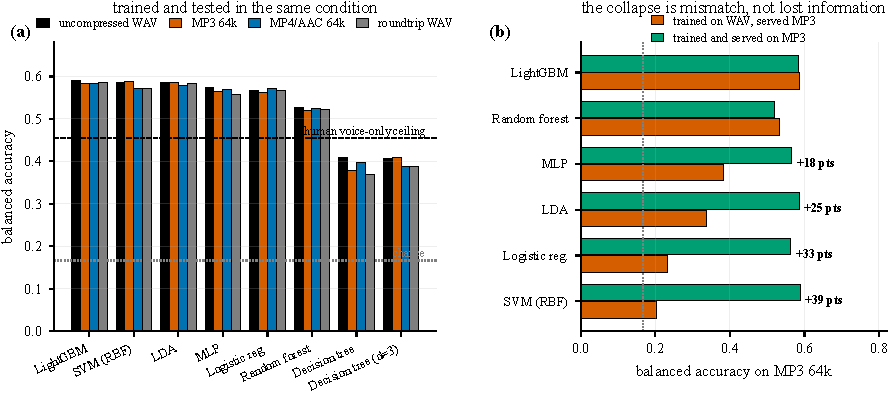
\includegraphics[width=\textwidth]{figs/fig_matched.pdf}
\caption{Matched-format training removes the damage that mismatch creates.
(a)~Every model, fitted and evaluated in the same condition, sits within 0.008
to 0.039 balanced accuracy of its uncompressed score --- including the two that
lose 33 and 38 points under mismatch. (b)~The same comparison on MP3 only.
The affective information survives \SI{64}{\kilo\bit\per\second} coding; what
fails is the mismatch between the distribution a model was fitted on and the one
it is served.}
\label{fig:matched}
\end{figure*}

The RBF-SVM scores $0.589$ on MP3 when trained on MP3, against $0.586$ on clean
audio --- a recovery of \textbf{38.6 balanced-accuracy points} over its
mismatched score of $0.203$. Logistic regression recovers 33.0 points, LDA 24.8,
the shallow MLP 18.2. No model's spread across the four conditions exceeds
0.039, and the two largest spreads belong to the single decision tree, whose
variance is high for reasons Section~\ref{sec:null} makes precise.

Three consequences follow.

\textbf{The codec does not remove the affective information.} If
\SI{64}{\kilo\bit\per\second} MP3 destroyed the acoustic correlates of emotion,
a model fitted on MP3 could not recover them. It does, to within three
thousandths of the clean-audio score. The catastrophic column of
Table~\ref{tab:crossformat} measures an artefact of deployment practice, not a
property of the codec.

\textbf{The tree family's advantage is an advantage under mismatch only.} Under
matched training, LightGBM's lead over the RBF-SVM is 0.008 on clean audio and
$-0.006$ on MP3. The robustness ordering of Section~\ref{sec:mismatch} is
entirely a statement about out-of-range inputs.

\textbf{The fix is format-specific, not general.} Trained on \ttf{mp4\_aac64}
and served MP3, the RBF-SVM falls to $0.167$ --- exactly chance. Matched-format
training immunises against the codec it was trained on and no other, which is
why Section~\ref{sec:neutralise}'s descriptor-level repair is the more practical
remedy when the delivery format is not known in advance.

\subsection{What the tree splits on, per condition}\label{sec:trees}
Accuracy parity does not entail evidential parity. Because the models are fitted
to named descriptors, the question can be asked directly: given audio that
supports the same accuracy, does the model reach it by asking the same
questions?

Fig.~\ref{fig:trees} and Table~\ref{tab:splits} show the top two levels of a
depth-3 entropy tree fitted independently on each condition. Every internal node
of all four trees is in Appendix~\ref{app:splits}.

\begin{figure*}[!t]
\centering
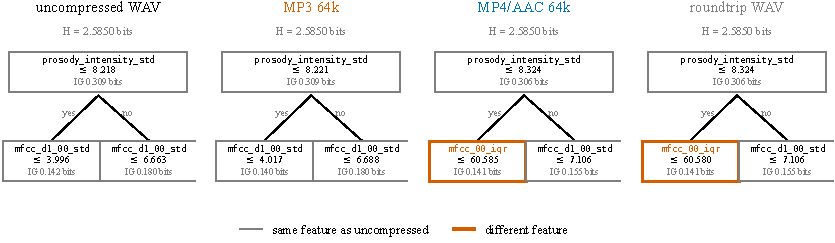
\includegraphics[width=\textwidth]{figs/fig_trees.pdf}
\caption{The top two levels of the depth-3 entropy tree, fitted separately on
each condition with the same actors and the same items. The root test is
codec-invariant in identity and near-invariant in threshold and information
gain. Divergence begins one level down, and it begins under AAC rather than
under MP3: the AAC and roundtrip trees abandon the frame-aligned delta
descriptor \ttf{mfcc\_d1\_00\_std} for the static dispersion measure
\ttf{mfcc\_00\_iqr}, which is what the \SI{32.68}{\milli\second} priming shift
predicts. AAC and roundtrip --- the same codec output through two containers ---
select identical descriptors with thresholds agreeing to four decimal places.}
\label{fig:trees}
\end{figure*}

\begin{table}[!t]
\caption{Root and depth-1 splits by condition, from the depth-3 entropy tree.
$H$ and IG are in bits (Eqs.~\ref{eq:entropy}--\ref{eq:ig}). \ttf{L} is the
branch taken when the root test is satisfied.}
\label{tab:splits}
\centering
\scriptsize
\setlength{\tabcolsep}{3pt}
\begin{tabular}{@{}llrr@{}}
\toprule
Condition & Descriptor & Threshold & IG\\
\midrule
\multicolumn{4}{@{}l@{}}{\textit{root} \quad $H=2.5850 bits=\log_2 6$}\\
\ttf{ref}            & \ttf{prosody\_intensity\_std} & 8.2184 & 0.3090\\
\ttf{mp3\_64}        & \ttf{prosody\_intensity\_std} & 8.2210 & 0.3090\\
\ttf{mp4\_aac64}     & \ttf{prosody\_intensity\_std} & 8.3241 & 0.3064\\
\ttf{roundtrip\_wav} & \ttf{prosody\_intensity\_std} & 8.3241 & 0.3064\\
\midrule
\multicolumn{4}{@{}l@{}}{\textit{depth 1, branch} \ttf{L}}\\
\ttf{ref}            & \ttf{mfcc\_d1\_00\_std} &  3.9965 & 0.1415\\
\ttf{mp3\_64}        & \ttf{mfcc\_d1\_00\_std} &  4.0175 & 0.1398\\
\ttf{mp4\_aac64}     & \textbf{\ttf{mfcc\_00\_iqr}} & 60.5853 & 0.1408\\
\ttf{roundtrip\_wav} & \textbf{\ttf{mfcc\_00\_iqr}} & 60.5802 & 0.1408\\
\bottomrule
\end{tabular}
\end{table}

Four observations, in increasing order of interest.

\textbf{The primary evidence is codec-invariant.} All four trees select
\ttf{prosody\_intensity\_std} at the root and extract almost exactly the same
information from it: 0.3090 bits under WAV and MP3, 0.3064 under AAC. Whatever
coding does to this feature space, it does not change the single most
discriminative question about a clip.

\textbf{The threshold moves, and it moves with the mechanism.} MP3 shifts the
root threshold by 0.03\,\% ($8.2184\rightarrow8.2210$); AAC shifts it by
1.29\,\% ($\rightarrow8.3241$). Intensity standard deviation is computed over
frames, and AAC's priming adds \SI{32.68}{\milli\second} of near-silent lead-in
to every clip, which raises the dispersion of the intensity contour. The tree
compensates by raising its threshold. This is the padding mechanism of
Fig.~\ref{fig:signal}(c) surfacing as a number in a decision rule.

\textbf{Divergence appears at depth 1, under AAC and not under MP3.} The
uncompressed and MP3 trees both ask about \ttf{mfcc\_d1\_00\_std}, the standard
deviation of the first temporal derivative of MFCC-0. The AAC and roundtrip
trees abandon it for \ttf{mfcc\_00\_iqr}, a \emph{static} dispersion measure of
the same coefficient. That is precisely what a frame-alignment perturbation
should do: it corrupts derivatives while leaving the distribution of the
underlying contour intact, so the tree switches from a temporal statistic to a
positional one at almost identical information gain (0.1408 vs 0.1415 bits).
The model finds an equally good question that the codec has not damaged.

\textbf{The container control reproduces at the structural level.}
\ttf{mp4\_aac64} and \ttf{roundtrip\_wav} carry the same codec output through
different containers. Their trees select identical descriptors at every node of
the top two levels, with thresholds agreeing to $8.3241$ vs $8.3241$ at the root
and $60.5853$ vs $60.5802$ at depth 1. Two conditions that differ only in
container produce the same model; two conditions that differ in codec do not.
The container/codec distinction, previously visible only as a difference in
accuracy, is here visible as a difference in the learned decision rule.

\subsection{Null calibration of the importance ranking}\label{sec:null}
The obvious next step is to compare the models' full importance rankings across
conditions, and the obvious result is dramatic: the tree's top-25 descriptors
under MP3 share only 12 members with its top-25 under WAV, and the rank
correlation over the descriptors either tree uses is $\rho=0.017$ --- no
relationship at all. Read naively, coding has almost completely rewritten what
the model considers important.

That reading is not supportable, and establishing why is this paper's
methodological contribution. A decision tree's deep importance ranking is a
fragile object. We measure three floors, all on the estimator that produced the
effect.

\begin{table}[!t]
\caption{Null calibration for the decision tree's importance ranking. Rows above
the rule are manipulations carrying no coding information; rows below are the
coding conditions. $\rho$ is Spearman rank correlation over the descriptors at
least one of the two fits actually used.}
\label{tab:null}
\centering
\scriptsize
\setlength{\tabcolsep}{4pt}
\begin{tabular}{@{}lccl@{}}
\toprule
Comparison & top-25 kept & $\rho$ & What it varies\\
\midrule
Tie-breaking      & 23.5 & $+0.946$ & estimator only; data fixed\\
Actor bootstrap   & \phantom{0}8.0 & $-0.200$ & training actors; codec fixed\\
Container re-wrap & 16.0 & $+0.184$ & decode path; codec output fixed\\
\midrule
MP3 @ 64k         & 12.0 & $+0.017$ & codec\\
MP4/AAC @ 64k     & \phantom{0}9.0 & $-0.082$ & codec\\
Roundtrip WAV     & 10.0 & $-0.123$ & codec\\
\bottomrule
\end{tabular}
\end{table}

Table~\ref{tab:null} and Fig.~\ref{fig:nullcal}(a) show why the naive reading
fails. Resampling \emph{which actors} the tree is fitted on --- with the codec
held fixed at uncompressed --- retains only 8.0 of 25 descriptors, worse than
any codec condition. Marginally compared, every codec effect sits inside the
sampling floor, and no codec claim can be made at all.

\begin{figure*}[!t]
\centering
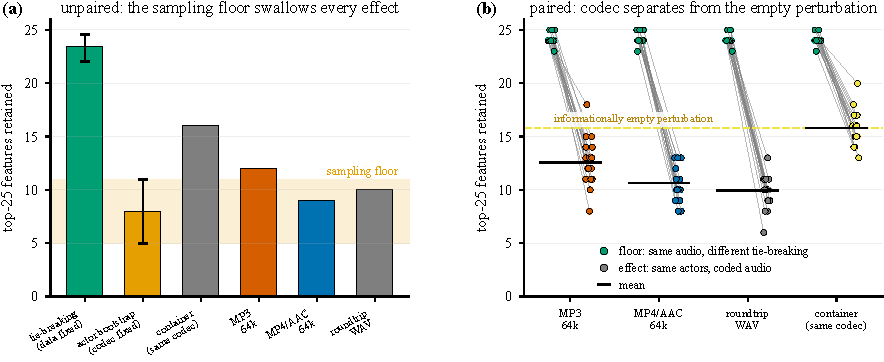
\includegraphics[width=\textwidth]{figs/fig_nullcal.pdf}
\caption{A codec effect on a feature-importance ranking is uninterpretable
without a null. (a)~Compared marginally, the actor-resampling floor is so wide
that every codec effect falls inside it. (b)~Measured \emph{inside} the same
resampled training set --- 20 draws of 51 of the 60 training actors, with the
floor and the effect computed on the same draw --- the codec effect separates
cleanly. The decisive control is the rightmost group: an informationally empty
container re-wrap already costs 8.4 of 25 descriptors, so only the gap between
that line and the codec bars is codec-attributable.}
\label{fig:nullcal}
\end{figure*}

The marginal comparison is the wrong one, because it varies two things at once:
the floor is estimated on one training set and the effect on another. We
therefore measure both \emph{inside the same draw}. On each of 20 draws, 51 of
the 60 training actors are sampled without replacement; the tree is fitted twice
on those actors' uncompressed audio under different tie-breaking, giving that
draw's floor, and once on the same actors' coded audio, giving that draw's
effect. Sampling variance is thereby held fixed by construction, and no actor is
duplicated.

\begin{table}[!t]
\caption{Paired within-draw comparison, 20 draws of 51 of 60 training actors.
The floor is a refit on the same actors' \emph{uncompressed} audio under
different tie-breaking. Wilcoxon signed-rank on the paired per-draw difference.}
\label{tab:paired}
\centering
\scriptsize
\setlength{\tabcolsep}{4pt}
\begin{tabular}{@{}lccc@{}}
\toprule
& top-25 kept & $\rho$ & $p$ vs.\ floor\\
\midrule
\textit{floor} (same audio, refit) & \textit{24.15} & $+0.958$ & ---\\
\midrule
Container re-wrap (empty)          & 15.80 & $+0.196$ & $8.1\times10^{-5}$\\
MP3 @ 64k                          & 12.55 & $-0.068$ & $8.4\times10^{-5}$\\
MP4/AAC @ 64k                      & 10.65 & $-0.137$ & $8.3\times10^{-5}$\\
Roundtrip WAV                      & \phantom{0}9.95 & $-0.126$ & $7.9\times10^{-5}$\\
\bottomrule
\end{tabular}
\end{table}

Table~\ref{tab:paired} and Fig.~\ref{fig:nullcal}(b) give the result, and it has
three layers.

\textbf{The estimator is reproducible.} With the data fixed and only
tie-breaking varied, the tree retains 24.15 of 25 top descriptors
($\rho=0.958$). Whatever else is fragile, the fitting procedure is not.

\textbf{An informationally empty perturbation is expensive.} The container
re-wrap changes no codec information --- it is the same AAC bitstream, decoded
identically, differing only by one int16 requantisation whose median feature
effect is $7.6\times10^{-5}$ standardised units. It nonetheless costs
\textbf{8.35 of 25} top descriptors ($24.15\rightarrow15.80$,
$p=8.1\times10^{-5}$). A ranking that turns over by a third under a manipulation
that carries no information cannot be read as a description of what the model
needs.

\textbf{The codec effect is real but roughly two-fifths the size it appears.}
Against the empty-perturbation floor of 15.80, MP3 retains 12.55
($p=1.1\times10^{-3}$, $d_z=1.20$) and AAC 10.65 ($p=1.2\times10^{-4}$,
$d_z=2.39$). So of the 13.5 descriptors that AAC appears to displace relative to
a clean refit, 8.35 are attributable to generic perturbation sensitivity and
only 5.15 to the codec. A study reporting the raw figure would over-attribute by
a factor of about $2.6$.

The direction of the codec-specific component is consistent with
Section~\ref{sec:trees}: AAC displaces more than MP3 in the ranking
($10.65$ vs $12.55$, $p=4.2\times10^{-3}$, $d_z=0.84$, paired), which is the
reverse of the accuracy ordering under mismatch, where MP3 is catastrophic and
AAC mild. Coding that perturbs every temporal derivative slightly reorganises a
tree more than coding that blows out one band the tree can simply threshold
around --- which is also what Section~\ref{sec:trees} shows structurally, since
it is the AAC tree and not the MP3 tree that replaces its depth-1 descriptor.

\subsection{Post-hoc attribution and its disagreements}
Attribution was computed on the held-out speakers using TreeSHAP for the
ensembles~\cite{lundberg2020treeshap}, LinearSHAP for the linear models, LIME
for local surrogates~\cite{ribeiro2016lime}, permutation importance, partial
dependence, a depth-4 global surrogate tree, and, for the network, six methods
from Captum~\cite{kokhlikyan2020captum}: Saliency, Input$\times$Gradient,
Integrated Gradients~\cite{sundararajan2017ig},
DeepLIFT~\cite{shrikumar2017deeplift}, GradientSHAP and Feature Ablation.

\subsubsection{Convergent evidence across families}
On uncompressed audio, five model families and four attribution algorithms
select the same acoustic evidence. The top SHAP descriptors for XGBoost and
LightGBM are identical in the first five (\ttf{mfcc\_d1\_00\_std},
\ttf{mfcc\_d2\_00\_std}, \ttf{duration\_s}, \ttf{prosody\_intensity\_std},
\ttf{mfcc\_00\_std}); the decision tree leads with
\ttf{prosody\_intensity\_std}, matching its root split; and all six gradient
methods on the network return \ttf{mfcc\_d1\_00\_std},
\ttf{mfcc\_d2\_00\_std}, \ttf{prosody\_cpps} and \ttf{duration\_s}. The two
leaders are the standard deviations of the first and second derivative of
MFCC-0 --- \emph{how variable the rate of change of overall loudness is} --- a
direct formalisation of vocal agitation.

Attribution mass is spread across families rather than concentrated
(Table~\ref{tab:famshare}), and the pattern matches the mutual-information
result of Section~\ref{sec:features}: MFCCs hold 55\,\% of the columns and take
roughly 55\,\% of the attribution, so they carry no per-descriptor advantage.
The single decision tree is the outlier, leaning harder on prosody --- which is
what makes it readable and also what caps its accuracy.

\begin{table}[!t]
\caption{Share of total attribution mass by descriptor family, on uncompressed
audio. Column share is the proportion of the 436 descriptors each family
contributes. SHAP except the ANN, which uses integrated gradients.}
\label{tab:famshare}
\centering
\scriptsize
\setlength{\tabcolsep}{4pt}
\begin{tabular}{@{}lccccc@{}}
\toprule
Model & MFCC & spectral & prosody & chroma & global\\
\midrule
\textit{column share} & \textit{0.550} & \textit{0.261} & \textit{0.128} & \textit{0.055} & \textit{0.005}\\
\midrule
XGBoost              & 0.566 & 0.207 & 0.178 & 0.033 & 0.016\\
LightGBM             & 0.550 & 0.209 & 0.189 & 0.030 & 0.021\\
Random forest        & 0.438 & 0.315 & 0.205 & 0.032 & 0.011\\
Decision tree        & 0.436 & 0.183 & \textbf{0.306} & 0.034 & 0.041\\
Logistic regression  & 0.471 & 0.306 & 0.156 & 0.062 & 0.005\\
ANN (int.\ grad.)    & 0.542 & 0.238 & 0.153 & 0.057 & 0.009\\
\bottomrule
\end{tabular}
\end{table}

Per-emotion attributions are acoustically sensible. CPPS, a breathiness
correlate, drives both sadness and neutrality; $F_0$ median drives fear; $F_2$
movement drives disgust; and loudness dynamics drive anger. The network was told
none of this.

\subsubsection{The methods disagree with each other}\label{sec:methods-disagree}
Fig.~\ref{fig:methods}(a) is the uncomfortable result. SHAP agrees closely with
a model's \emph{intrinsic} importance for the simpler models ($\rho=0.98$ for
both the decision tree and logistic regression), but LIME and permutation
importance are close to unrelated to it. On the decision tree, LIME and SHAP
rank descriptors at $\rho=0.008$ --- no relationship at all --- while still
sharing 10 of their top 20. This reproduces the disagreement problem Krishna et
al.~\cite{krishna2022disagreement} document, on a model simple enough that no
approximation error can be blamed.

\begin{figure*}[!t]
\centering
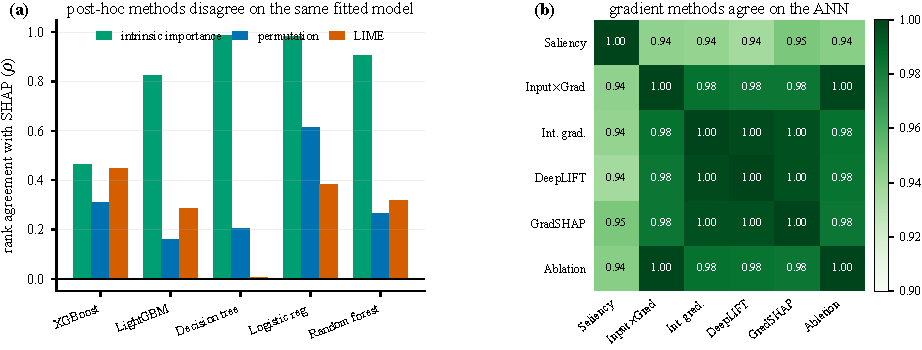
\includegraphics[width=\textwidth]{figs/fig_methods.pdf}
\caption{Explanation-method agreement, measured as Spearman rank correlation
over all 436 descriptors. (a)~Post-hoc methods applied to the same fitted
tabular model. SHAP tracks intrinsic importance closely for the simpler models
but LIME and permutation importance are nearly unrelated to it; on the decision
tree, LIME and SHAP agree at $\rho=0.008$. (b)~The six gradient-family methods
applied to the network agree almost perfectly ($\rho\geq0.94$ pairwise), which
shows that the disagreement in (a) is a property of the method families rather
than of this feature space.}
\label{fig:methods}
\end{figure*}

Panel~(b) sharpens the point rather than softening it. The six gradient-family
methods on the network agree almost perfectly ($\rho\geq0.94$ pairwise, with
Integrated Gradients and DeepLIFT at $0.998$). High agreement within a method
family is therefore not evidence of correctness --- these methods share a
mathematical lineage, and their consensus reflects that lineage. The practical
consequence is that a single-method claim about which acoustic descriptors
matter is not reproducible across methods. Only descriptors surviving all four
independent views should be reported as robust; here that set is
\ttf{mfcc\_d1\_00\_std}, \ttf{prosody\_intensity\_std}, \ttf{duration\_s},
\ttf{prosody\_cpps} and \ttf{prosody\_f0\_median}.

Two further calibrations belong with this result. A depth-4 global surrogate
reproduces its target model's predictions only 57 to 74\,\% of the time (random
forest 73.9\,\%, LightGBM 63.4\,\%, XGBoost 62.1\,\%, SVM 58.7\,\%, logistic
regression 57.1\,\%), so surrogate rules summarise a majority of a model, not a
model; reporting them without their fidelity would overstate what has been
explained. And the network's attributions pass the Adebayo model-randomisation
check (Fig.~\ref{fig:sanity}): correlation between attributions from the trained
network and a randomly initialised one of identical architecture ranges from
$-0.011$ to $0.206$ across all six methods. These explanations describe the
trained model, not merely the input distribution.

\begin{figure}[!t]
\centering
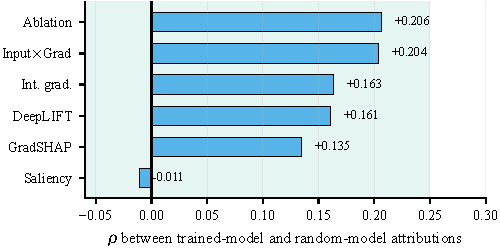
\includegraphics[width=\columnwidth]{figs/fig_sanity.pdf}
\caption{Model-randomisation sanity check~\cite{adebayo2018sanity} for the six
gradient-family methods. A method whose attributions correlate with those of a
randomly initialised network of identical architecture is describing the input
distribution rather than the model. All six sit near zero, so the failure mode
does not apply here.}
\label{fig:sanity}
\end{figure}

\subsubsection{An estimator that failed loudly}\label{sec:kernelshap}
The RBF-SVM has no exact explainer, so it was given KernelSHAP with 100 sampled
coalitions over 436 descriptors. KernelSHAP fits a weighted least-squares
regression with one unknown per descriptor; with 100 coalitions for 436 unknowns
that system is rank-deficient, and the result diverged --- maximum mean
$|$SHAP$|$ of $2.1\times10^{12}$ against a median of $5.3\times10^{-4}$, with
entire descriptor families assigned exactly zero. A cheap tell that this had
gone wrong: a well-behaved additive attribution over 7{,}441 clips does not
assign a whole family exactly 0.000.

The SVM's KernelSHAP ranking is excluded from every conclusion in this paper as
an estimation artefact, and the implementation now raises when the coalition
budget does not exceed the descriptor count. The SVM contributes accuracy and
robustness results but no attribution row; its trustworthy views are permutation
importance and LIME, whose top descriptors reproduce the consensus every other
model reaches.

\subsection{Attribution stability under coding}\label{sec:stability}
Table~\ref{tab:stability} reports SHAP rank stability under train/serve
mismatch. Tree and linear attributions barely move; the network's move
substantially.

\begin{table}[!t]
\caption{Attribution stability under mismatch: Spearman $\rho$ over all 436
descriptors against the uncompressed condition, with the number of top-25
descriptors retained in parentheses. SHAP for all rows except the ANN, which
uses integrated gradients.}
\label{tab:stability}
\centering
\scriptsize
\setlength{\tabcolsep}{3pt}
\begin{tabular}{@{}lcccc@{}}
\toprule
Model & \ttf{mp3\_64} & \ttf{mp4\_aac64} & \ttf{roundtrip} & $\Delta$ acc.\ MP3\\
\midrule
Decision tree       & 0.995 (24) & 0.988 (21) & 0.988 (21) & $-0.009$\\
XGBoost             & 0.991 (25) & 0.984 (22) & 0.984 (22) & $+0.004$\\
Random forest       & 0.990 (25) & 0.976 (25) & 0.975 (25) & $-0.003$\\
LightGBM            & 0.988 (23) & 0.983 (22) & 0.982 (22) & $-0.005$\\
Logistic regression & 0.987 (22) & 0.942 (21) & 0.941 (21) & $\mathbf{-0.334}$\\
ANN (int.\ grad.)   & \textbf{0.677 (11)} & 0.891 (16) & 0.887 (16) & $-0.246$\\
\bottomrule
\end{tabular}
\end{table}

These rows measure something different from Section~\ref{sec:null}, and the
distinction matters. Here the \emph{model is fixed} and only its input changes,
so the comparison is between two attributions of one fitted object. In
Section~\ref{sec:null} the model is refitted, so the comparison is between two
learned objects. The first is stable because a fitted tree's split structure
does not move when you feed it slightly different numbers; the second is not,
because the fitting procedure can reach an equally good structure by a different
route.

Even so, the accuracy figure understates the attribution figure throughout.
XGBoost loses 2.2 accuracy points on AAC and still swaps 3 of its top 25; the
network loses 8.7 points and swaps 9. An accuracy-only benchmark would call the
first negligible and the second modest.

What replaces what is readable only because the descriptors are named. Under
MP3 the descriptors \emph{entering} the network's top 25 are almost all encoder
artefacts --- \ttf{spectral\_flatness} in five statistics, plus
\ttf{spectral\_contrast\_6\_mean} --- while those \emph{leaving} are genuine
voice-quality and prosodic measures: \ttf{prosody\_cpps},
\ttf{prosody\_f0\_skew}, \ttf{prosody\_f2\_mean}, \ttf{prosody\_f2\_std},
\ttf{prosody\_f3\_bw\_median}. Under mismatch, the model stops listening to the
voice and starts listening to the encoder.

\subsubsection{A blind spot in global attribution metrics}\label{sec:blindspot}
The logistic regression row of Table~\ref{tab:stability} is the most important
negative result in this paper. Its SHAP ranking is essentially unchanged under
MP3 ($\rho=0.987$, 22 of 25 top descriptors retained) while its balanced
accuracy collapses from $0.567$ to $0.233$. The coefficients did not change;
only the inputs went out of range, and a global mean-$|$SHAP$|$ ranking is
largely blind to that.

This is a caution about the method, not about the model. \textbf{A global
attribution-stability metric can report ``nothing changed'' while the classifier
has effectively stopped working.} Any deployment that monitors explanation
stability as a proxy for model health must pair it with input-range monitoring
or local, per-instance attribution; the global ranking alone will not raise the
alarm.

\subsection{Diagnosis and repair}\label{sec:neutralise}
Because the descriptors are named, the mismatch failure is not merely observable
but addressable. Descriptors were ranked by how far each codec moves them in
units of \emph{training} standard deviation, then progressively replaced with
training medians in both the compressed and the clean test set --- the clean
column controlling for whatever real signal the masking itself destroys.

\begin{figure}[!t]
\centering

\includegraphics[width=\columnwidth]{figs/fig_neutralise.pdf}
\caption{Neutralisation on MP3 at \SI{64}{\kilo\bit\per\second}: replacing the
most codec-shifted descriptors with their training medians. Masking one
descriptor recovers almost the entire collapse for every affected model; the
tree models were never affected and are flat throughout. Beyond roughly 20
descriptors the masking begins to destroy real evidence. On uncompressed audio
the same masking costs nothing out to 20 descriptors, confirming these columns
were never load-bearing evidence.}
\label{fig:neutralise}
\end{figure}

\begin{table}[!t]
\caption{Balanced accuracy on MP3 as the most codec-shifted descriptors are
replaced by training medians. Italic row: the model's own clean-audio score.
Tree columns are flat because they had nothing to recover.}
\label{tab:neutralise}
\centering
\footnotesize
\setlength{\tabcolsep}{4pt}
\begin{tabular}{@{}lcccccc@{}}
\toprule
Masked & SVM & Log.\ reg. & ANN & MLP & XGBoost & Dec.\ tree\\
\midrule
\textit{clean} & \textit{0.586} & \textit{0.567} & \textit{0.599} & \textit{0.574} & \textit{0.582} & \textit{0.391}\\
0  & 0.203 & 0.233 & 0.354 & 0.383 & 0.586 & 0.382\\
\textbf{1} & \textbf{0.578} & \textbf{0.502} & \textbf{0.580} & \textbf{0.552} & 0.581 & 0.382\\
2  & 0.583 & 0.529 & 0.587 & 0.554 & 0.581 & 0.391\\
3  & 0.579 & \textbf{0.562} & \textbf{0.595} & 0.565 & 0.580 & 0.391\\
10 & 0.575 & 0.539 & 0.589 & 0.562 & 0.582 & 0.394\\
80 & 0.551 & 0.435 & 0.574 & 0.523 & 0.564 & 0.396\\
\bottomrule
\end{tabular}
\end{table}

The single masked descriptor is \ttf{spectral\_contrast\_6\_mean}. Masking it
alone recovers 98\,\% of the RBF-SVM's 38.3-point loss and 92\,\% of the
network's 24.6-point loss; three descriptors bring logistic regression to
$0.562$ against its $0.567$ clean-audio score.

Two controls make this a diagnosis rather than a coincidence. On uncompressed
audio the identical masking costs nothing out to 20 descriptors --- the
network's clean control sits at $0.607$--$0.609$, marginally \emph{above} its
$0.599$ unmasked baseline --- so these columns were never load-bearing evidence;
they were the channel through which the encoder's fingerprint entered the model.
And the AAC case behaves as its different mechanism predicts: no single
descriptor dominates, with the network's best recovery arriving at 10
descriptors masked ($0.513\rightarrow0.560$) and the SVM's at 40
($0.499\rightarrow0.542$).

The diagnosis is therefore covariate shift on a small set of identifiable
descriptors, not loss of emotional information --- which is exactly what
Section~\ref{sec:matched} establishes independently, by a different route.

\section{Discussion}

\subsection{Three questions that are usually one}
This study separates three things that a single accuracy number conflates.
\emph{Does the codec destroy the information?} No: matched-format training
recovers 38.6 points and lands within 0.003 of the clean score.
\emph{Does the codec break deployed models?} Severely, if they consume
descriptor magnitudes and were fitted on clean audio.
\emph{Does the codec change what the model learns?} Yes, but by much less than
the raw numbers suggest, and only a properly nulled comparison can say by how
much.

An evaluation reporting only the second question --- which is what
cross-format benchmarking does --- would conclude that
\SI{64}{\kilo\bit\per\second} MP3 is unusable for SER. The first question shows
that conclusion is about the pipeline, not the codec.

\subsection{Null calibration is not optional}
The container re-wrap changes no coding information and still turns over a third
of the tree's top-25 ranking. Any claim of the form ``manipulation $M$ changed
which features the model uses'' is therefore uninterpretable without a
perturbation matched in every respect except informational content. We propose
this as standard practice for feature-attribution claims in affective computing.
The cost is one additional condition and one additional model fit; the benefit
is that the claim becomes falsifiable, and in our case that it shrinks by a
factor of 2.6 rather than being reported at face value.

The paired design matters as much as the null itself. Compared marginally, the
actor-resampling floor was wide enough to swallow every codec effect
(Fig.~\ref{fig:nullcal}(a)) and we would have reported nothing. Measuring floor
and effect inside the same resampled training set removes sampling variance by
construction and recovers a clean answer.

\subsection{What a threshold buys, and what it does not}
Under mismatch, axis-aligned models are almost perfectly robust to a
$38\sigma$ excursion, because a threshold test is invariant to how far past the
threshold a value lands. That is a real and cheap engineering advantage. But
Section~\ref{sec:matched} shows it disappears under matched training, and
Section~\ref{sec:null} shows the same models' learned structure is \emph{more}
sensitive to a small diffuse perturbation than a large concentrated one. The
threshold protects the decision, not the evidence.

\subsection{Auditing and the archive problem}
Per-instance rationales are increasingly surfaced to operators and auditors. Our
results indicate that such rationales are not invariant across a transcoding
step that may leave the decision invariant. Where an audit is conducted on
archived compressed material while inference runs on uncompressed input --- or
the converse --- the decisions will agree while the explanations will not. An
explanation is not reproducible unless the delivery format is part of the
record, and to our knowledge no SER benchmark currently reports it.

\subsection{What named descriptors buy}
The repair in Section~\ref{sec:neutralise} has no analogue in a system whose
front end is learned. Identifying \ttf{spectral\_contrast\_6\_mean} as the
contaminated channel required attribution over units with acoustic meaning;
neutralising it required reaching into the representation. So did reading the
codec's frame-alignment mechanism off a decision threshold
(Section~\ref{sec:trees}).

This is a narrower claim than Rudin's~\cite{rudin2019stop}. We are not arguing
that interpretable models should replace strong ones ---
Table~\ref{tab:leaderboard} shows the single interpretable model in our zoo
costing a third of achievable performance, and the best model overall is a
neural network. We are arguing that a \emph{named-descriptor front end} retains
a diagnostic and repair capability that end-to-end pipelines lack, and that in
codec-heterogeneous deployments this capability has measurable value: 98\,\% of
a 38-point loss, recovered by masking one column.

\section{Limitations}
\begin{enumerate}
\item \textbf{Acted, not spontaneous, emotion.} CREMA-D actors perform
prescribed emotions on 12 fixed sentences. Absolute accuracies do not transfer
to spontaneous speech, and the human voice-only ceiling of 45.5\,\% shows the
labels are themselves only loosely recoverable from audio.

\item \textbf{One split, not repeated cross-validation, for the headline
tables.} Tables~\ref{tab:leaderboard}--\ref{tab:matched} come from a single
deterministic 60/11/20 actor partition. Differences of a point or two should not
be over-read. The null-calibration analysis of Section~\ref{sec:null} does
resample (20 draws), and is the only place we make a claim that depends on
resampling.

\item \textbf{Two codecs, one bitrate.} Only \SI{64}{\kilo\bit\per\second} MP3
and AAC were tested. The MP3 mismatch result is severe partly \emph{because}
\SI{64}{\kilo\bit\per\second} is aggressive for that codec; higher bitrates
would likely show a gradient, and Opus --- now the dominant conversational codec
--- is untested.

\item \textbf{Summary statistics discard time.} Every frame contour is collapsed
to eight order statistics, so no attribution here localises \emph{when} in a
clip the evidence sits. The AAC padding mechanism is inferred from duration and
from which descriptors move, not observed directly in time.

\item \textbf{The container control is not a perfect null.} \ttf{roundtrip\_wav}
differs from \ttf{mp4\_aac64} by an int16 requantisation, so it is an
\emph{almost} empty perturbation rather than an exactly empty one. It is
conservative in the right direction --- a truly empty perturbation would have a
lower floor and make the codec effects look larger --- but a bit-exact container
null would be a stronger instrument.

\item \textbf{The null calibration covers one estimator.} Section~\ref{sec:null}
calibrates the decision tree, chosen because it is the paper's readable model
and the one whose ranking is most obviously fragile. Whether ensemble or
gradient attributions need floors of the same size is not established here,
though Table~\ref{tab:stability}'s fixed-model comparison suggests they are more
stable.

\item \textbf{Attribution comparisons are global.} Spearman $\rho$ and top-$k$
overlap over mean-$|$attribution$|$ are coarse instruments, and
Section~\ref{sec:blindspot} shows they can miss a total accuracy collapse. A
local, per-instance stability analysis would be stronger and is not attempted.

\item \textbf{Speaker-dominance limits what importance rankings can mean.} With
mean $\eta^2=0.178$ for speaker against $0.098$ for emotion, a substantial part
of any importance ranking describes which voices are in the training set. The
actor-bootstrap floor in Table~\ref{tab:null} quantifies this and it is large.

\item \textbf{Exploratory, not confirmatory.} The per-condition and
null-calibration analyses were designed after inspecting the cross-format
results. Confirmatory status requires preregistered replication.
\end{enumerate}

\section{Future Work}
Three directions follow from specific results. A bit-exact container null ---
achievable by comparing two lossless containers carrying identical PCM --- would
tighten the floor of Section~\ref{sec:null} and is cheap. Extending the null
calibration to SHAP and integrated-gradients rankings under refitting would
establish whether the fragility we document is specific to trees or general to
feature attribution. And a bitrate ladder, with Opus alongside MP3 and AAC,
would turn the two-point comparison in Section~\ref{sec:trees} into a
dose-response curve for structural displacement.

Beyond emotion, speaker identity, vocal stress and voice quality are carried by
precisely the spectral detail perceptual coding discards, and the matched-format
result may not transfer: a task whose evidence lives in the top octave has less
to fall back on than one whose evidence lives in loudness dynamics.

\section{Conclusion}
We asked whether perceptual audio coding changes what a speech emotion model
relies on, using models whose evidence is a named acoustic descriptor rather
than a latent dimension.

Coding does not remove the affective information: a kernel machine that scores
0.203 on MP3 when fitted to clean audio scores 0.589 when fitted to MP3 itself,
against 0.586 on clean audio. The catastrophic cross-format losses in the
literature and in our own Table~\ref{tab:crossformat} are train/serve mismatch,
and they are repairable either by matched training or by neutralising a single
contaminated descriptor.

What coding does change is the structure the model learns. An entropy tree keeps
the same root question in every condition and extracts the same information from
it, but AAC moves the root threshold by 1.3\,\% and replaces the depth-1
descriptor with one its frame-alignment perturbation leaves intact --- while the
same two conditions carrying identical codec output through different containers
produce identical trees.

The size of that change is easy to overstate, and the discipline that prevents
it is the paper's most transportable result. An informationally empty container
re-wrap already displaces 8.35 of a tree's 25 most important descriptors. Only
the gap beyond that floor --- 3.25 descriptors for MP3, 5.15 for AAC --- is
codec-attributable. We would ask reviewers of affective computing systems to
require, alongside any claim that an intervention changed a model's explanation,
the divergence induced by an intervention carrying no information. Without it,
the claim cannot be evaluated; with it, ours shrinks by a factor of two and a
half and becomes defensible.

\section*{Data Availability Statement}
CREMA-D is publicly available from its authors under the terms stated
in~\cite{cao2014cremad}. All derived artefacts are released with this paper: the
stimulus construction scripts and condition manifests, the JSON schema of the
436-descriptor table over 29{,}768 rendered files, the per-condition and
null-calibration result files, and the JSON/CSV files from which every table and
figure is generated. The figure- and appendix-generation scripts read only these
committed artefacts and hard-code no numbers. The feature table itself
(\SI{243}{\mega\byte}) and the rendered audio are regenerable from the committed
extraction code and configuration.

\section*{Ethics Declaration}
This study involves no human subjects and no personally identifying data. It
uses a published corpus of consenting professional actors performing scripted
sentences, collected and released for research use by its original authors under
their own ethical approval~\cite{cao2014cremad}. No new recordings were made. We
note that speech emotion recognition is a dual-use technology; the findings here
concern robustness and explanation validity and are, if anything, cautionary
about deploying such systems on heterogeneous audio without format-aware
validation. Nothing here should be read as evidence that automatic emotion
inference is accurate, fair, or appropriate in consequential settings.

\section*{Author Contributions (CRediT)}
\textbf{Akshath~R:} Conceptualization, Methodology, Software, Validation, Formal
analysis, Investigation, Data curation, Writing --- original draft, Writing ---
review \& editing, Visualization, Project administration.

\section*{Conflict of Interest Statement}
The author declares no competing financial or non-financial interests.

\section*{Funding}
This research received no specific grant from any funding agency in the public,
commercial, or not-for-profit sectors. Compute costs were borne by the author.

\section*{Declaration of Generative AI Use}
Generative AI tools were used to assist with code implementation, figure
generation, and manuscript drafting. All experimental design decisions, all
analyses, and all interpretations are the author's. Every numerical value
reported was produced by the committed pipeline and traced to its source
artefact. The author takes full responsibility for the content.

% GENERATED BY make_appendix.py -- DO NOT EDIT BY HAND
\appendices

\section{Complete Feature Inventory}\label{app:features}

Every stimulus is reduced to 436 named columns. Frame-level contours are summarised by eight order statistics (mean, standard deviation, minimum, maximum, median, interquartile range, skewness, excess kurtosis). Descriptors marked with a shorter list are summarised only by those statistics, and scalars are already clip-level. Naming is \ttf{<family>\_<descriptor>\_<statistic>} throughout, which is what makes an attribution over a column a claim about an acoustic quantity.

Analysis frames are \SI{512}{point} FFT, \SI{400}{sample} window, \SI{160}{sample} hop at \SI{16}{\kilo\hertz}, which gives \SI{25}{\milli\second} windows every \SI{10}{\milli\second}. Praat measures use a \SIrange{75}{500}{\hertz} pitch range.

\subsection{Descriptors and their definitions}

\begin{table}[H]
\caption{Spectral descriptors. 114 columns of 436. ``all 8'' denotes the eight order statistics of Section~\ref{sec:features}: mean, standard deviation, minimum, maximum, median, IQR, skewness and excess kurtosis.}
\label{tab:app-spectral}
\centering\scriptsize\setlength{\tabcolsep}{3pt}
\begin{tabular}{@{}>{\raggedright\arraybackslash}p{2.05cm}>{\raggedright\arraybackslash}p{3.85cm}>{\raggedright\arraybackslash}p{1.20cm}r@{}}
\toprule
Descriptor & Definition & Stats & $n$\\
\midrule
Spectral centroid & First moment of the power spectrum. It is the frequency about which spectral energy is balanced. Correlates with perceived brightness. & all 8 & 8\\
Spectral bandwidth & Power-weighted second moment about the centroid. It measures how widely energy is spread in frequency. & all 8 & 8\\
Spectral roll-off (85\,\%) & Frequency below which 85\,\% of the frame's spectral energy lies. & all 8 & 8\\
Spectral roll-off (95\,\%) & As above at 95\,\%. Directly sensitive to codec low-pass behaviour. & all 8 & 8\\
Spectral flatness & Geometric mean of the magnitude spectrum divided by its arithmetic mean. It approaches 1 for noise-like frames and 0 for tonal ones, and it collapses when an encoder sets masked bins to zero. & all 8 & 8\\
Zero-crossing rate & Fraction of adjacent sample pairs with a sign change. It is a cheap proxy for voicing and frication. & all 8 & 8\\
Frame RMS energy & Root-mean-square magnitude per frame, which gives the loudness contour. & all 8 & 8\\
Spectral flux & Euclidean norm of the frame-to-frame difference of the magnitude spectrum. It measures how fast the spectrum is changing. & all 8 & 8\\
Spectral entropy & Shannon entropy of the power spectrum normalised to its own bin count (Eq.~\ref{eq:specent}). It is a scale-free measure of how evenly energy is distributed across frequency. & all 8 & 8\\
Spectral slope & Least-squares slope of magnitude regressed on frequency, per frame. This is the spectral tilt. & all 8 & 8\\
Band-energy ratios (8 bands) & Fraction of frame energy in each of 0--500, 500--1000, 1000--2000, 2000--3000, 3000--4000, 4000--5000, 5000--6000, 6000--8000\,Hz. Energy-normalised, so these describe spectral \emph{shape} rather than level. & mean, std & 16\\
High-frequency survival ratios & Fraction of frame energy above 4 and above 6\,kHz. The most direct probes of lossy-codec low-pass behaviour in the inventory. & mean, std & 4\\
Spectral contrast (7 sub-bands) & Per-band difference between spectral peaks and valleys in decibels. Band 6 covers 6--8\,kHz and is the single most codec-displaced column in the table (Section~\ref{sec:signal}). & mean, std & 14\\
\bottomrule
\end{tabular}
\end{table}

\begin{table}[H]
\caption{Cepstral descriptors. 240 columns of 436. ``all 8'' denotes the eight order statistics of Section~\ref{sec:features}: mean, standard deviation, minimum, maximum, median, IQR, skewness and excess kurtosis.}
\label{tab:app-mfcc}
\centering\scriptsize\setlength{\tabcolsep}{3pt}
\begin{tabular}{@{}>{\raggedright\arraybackslash}p{2.05cm}>{\raggedright\arraybackslash}p{3.85cm}>{\raggedright\arraybackslash}p{1.20cm}r@{}}
\toprule
Descriptor & Definition & Stats & $n$\\
\midrule
$\Delta$MFCC (20) & First-order temporal derivative of each MFCC, over a 9-frame window. & mean, std & 40\\
$\Delta\Delta$MFCC (20) & Second-order temporal derivative of each MFCC. & mean, std & 40\\
MFCC (20) & Discrete cosine transform of the log mel-filterbank energies, which is the standard SER front end. MFCC-0 tracks overall log energy, so its derivatives measure how fast loudness changes. & all 8 & 160\\
\bottomrule
\end{tabular}
\end{table}

\begin{table}[H]
\caption{Prosodic and voice-quality descriptors (Praat). 56 columns of 436. ``all 8'' denotes the eight order statistics of Section~\ref{sec:features}: mean, standard deviation, minimum, maximum, median, IQR, skewness and excess kurtosis.}
\label{tab:app-prosody}
\centering\scriptsize\setlength{\tabcolsep}{3pt}
\begin{tabular}{@{}>{\raggedright\arraybackslash}p{2.05cm}>{\raggedright\arraybackslash}p{3.85cm}>{\raggedright\arraybackslash}p{1.20cm}r@{}}
\toprule
Descriptor & Definition & Stats & $n$\\
\midrule
$F_0$ slope (mean $|\cdot|$) & Mean absolute first difference of the voiced $F_0$ contour, per second. It is the rate of pitch movement. & scalar & 1\\
Fundamental frequency $F_0$ & Praat autocorrelation pitch over voiced frames only. & all 8 & 8\\
Jitter (4 variants) & Cycle-to-cycle variation in glottal period: local, RAP, PPQ5, DDP. A perturbation measure of the voice source. & scalar & 4\\
Shimmer (6 variants) & Cycle-to-cycle variation in glottal amplitude: local, local\,dB, APQ3, APQ5, APQ11, DDA. APQ11 needs eleven consecutive periods and is the one column in the table with non-trivial missingness (11.3\,\%). & scalar & 6\\
Harmonics-to-noise ratio & Ratio of periodic to aperiodic energy in decibels. It correlates with hoarseness and breathiness. & mean, std, min, max, median & 5\\
Formant bandwidths $B_1$--$B_3$ & Median $-3$\,dB bandwidth of the first three formants (Burg estimator). & median & 1\\
Formants $F_1$--$F_5$ & Burg-estimator formant frequencies, which describe the vocal-tract filter. $F_2$ movement is the strongest single correlate of disgust in this corpus. & mean, std, median & 17\\
Intensity & Praat short-term intensity contour in decibels. Its standard deviation is among the top-ranked features for every model family in the study. & all 8 & 8\\
Voiced fraction & Proportion of frames with a defined $F_0$. & scalar & 1\\
Pause fraction & Complement of the voiced fraction. By definition it equals $1 -$ voiced fraction ($r = -1.00$). & scalar & 1\\
Voiced-segment count & Number of maximal runs of voiced frames. & scalar & 1\\
Voiced-segment rate & Voiced segments per second, which is a proxy for speech rate. & scalar & 1\\
Mean voiced-segment duration & Mean length in seconds of a voiced run. & scalar & 1\\
CPPS & Smoothed cepstral peak prominence, which is the standard acoustic correlate of breathy phonation. Drives both sadness and neutrality in every attribution method applied here. & scalar & 1\\
\bottomrule
\end{tabular}
\end{table}

\begin{table}[H]
\caption{Chroma descriptors. 24 columns of 436. ``all 8'' denotes the eight order statistics of Section~\ref{sec:features}: mean, standard deviation, minimum, maximum, median, IQR, skewness and excess kurtosis.}
\label{tab:app-chroma}
\centering\scriptsize\setlength{\tabcolsep}{3pt}
\begin{tabular}{@{}>{\raggedright\arraybackslash}p{2.05cm}>{\raggedright\arraybackslash}p{3.85cm}>{\raggedright\arraybackslash}p{1.20cm}r@{}}
\toprule
Descriptor & Definition & Stats & $n$\\
\midrule
Chroma (12 pitch classes) & Energy folded onto the twelve semitone pitch classes. Tuning is pinned to 0 rather than estimated, because an estimated tuning could itself shift under compression and become part of the effect being measured. & mean, std & 24\\
\bottomrule
\end{tabular}
\end{table}

\begin{table}[H]
\caption{Global descriptors. 2 columns of 436. ``all 8'' denotes the eight order statistics of Section~\ref{sec:features}: mean, standard deviation, minimum, maximum, median, IQR, skewness and excess kurtosis.}
\label{tab:app-global}
\centering\scriptsize\setlength{\tabcolsep}{3pt}
\begin{tabular}{@{}>{\raggedright\arraybackslash}p{2.05cm}>{\raggedright\arraybackslash}p{3.85cm}>{\raggedright\arraybackslash}p{1.20cm}r@{}}
\toprule
Descriptor & Definition & Stats & $n$\\
\midrule
Clip duration & Decoded duration in seconds. Rises by 32.68\,ms under AAC encoder priming, uniformly across every clip. & scalar & 1\\
Peak amplitude & Maximum absolute sample value after loudness normalisation. & scalar & 1\\
\bottomrule
\end{tabular}
\end{table}

\subsection{Enumerated column names}

The complete inventory, in the order the extractor emits it.

\begin{table*}[!tp]
\caption{Spectral descriptors: all 114 column names.}
\label{tab:app-list-spectral}
\centering\tiny\setlength{\tabcolsep}{3pt}
\begin{tabular}{@{}llll@{}}
\toprule
\texttt{spectral\_centroid\_mean} & \texttt{spectral\_rolloff95\_iqr} & \texttt{spectral\_flux\_min} & \texttt{spectral\_band\_2000\_3000\_std}\\
\texttt{spectral\_centroid\_std} & \texttt{spectral\_rolloff95\_skew} & \texttt{spectral\_flux\_max} & \texttt{spectral\_band\_3000\_4000\_mean}\\
\texttt{spectral\_centroid\_min} & \texttt{spectral\_rolloff95\_kurt} & \texttt{spectral\_flux\_median} & \texttt{spectral\_band\_3000\_4000\_std}\\
\texttt{spectral\_centroid\_max} & \texttt{spectral\_flatness\_mean} & \texttt{spectral\_flux\_iqr} & \texttt{spectral\_band\_4000\_5000\_mean}\\
\texttt{spectral\_centroid\_median} & \texttt{spectral\_flatness\_std} & \texttt{spectral\_flux\_skew} & \texttt{spectral\_band\_4000\_5000\_std}\\
\texttt{spectral\_centroid\_iqr} & \texttt{spectral\_flatness\_min} & \texttt{spectral\_flux\_kurt} & \texttt{spectral\_band\_5000\_6000\_mean}\\
\texttt{spectral\_centroid\_skew} & \texttt{spectral\_flatness\_max} & \texttt{spectral\_entropy\_mean} & \texttt{spectral\_band\_5000\_6000\_std}\\
\texttt{spectral\_centroid\_kurt} & \texttt{spectral\_flatness\_median} & \texttt{spectral\_entropy\_std} & \texttt{spectral\_band\_6000\_8000\_mean}\\
\texttt{spectral\_bandwidth\_mean} & \texttt{spectral\_flatness\_iqr} & \texttt{spectral\_entropy\_min} & \texttt{spectral\_band\_6000\_8000\_std}\\
\texttt{spectral\_bandwidth\_std} & \texttt{spectral\_flatness\_skew} & \texttt{spectral\_entropy\_max} & \texttt{spectral\_hf\_ratio\_4000\_mean}\\
\texttt{spectral\_bandwidth\_min} & \texttt{spectral\_flatness\_kurt} & \texttt{spectral\_entropy\_median} & \texttt{spectral\_hf\_ratio\_4000\_std}\\
\texttt{spectral\_bandwidth\_max} & \texttt{spectral\_zcr\_mean} & \texttt{spectral\_entropy\_iqr} & \texttt{spectral\_hf\_ratio\_6000\_mean}\\
\texttt{spectral\_bandwidth\_median} & \texttt{spectral\_zcr\_std} & \texttt{spectral\_entropy\_skew} & \texttt{spectral\_hf\_ratio\_6000\_std}\\
\texttt{spectral\_bandwidth\_iqr} & \texttt{spectral\_zcr\_min} & \texttt{spectral\_entropy\_kurt} & \texttt{spectral\_contrast\_0\_mean}\\
\texttt{spectral\_bandwidth\_skew} & \texttt{spectral\_zcr\_max} & \texttt{spectral\_slope\_mean} & \texttt{spectral\_contrast\_0\_std}\\
\texttt{spectral\_bandwidth\_kurt} & \texttt{spectral\_zcr\_median} & \texttt{spectral\_slope\_std} & \texttt{spectral\_contrast\_1\_mean}\\
\texttt{spectral\_rolloff85\_mean} & \texttt{spectral\_zcr\_iqr} & \texttt{spectral\_slope\_min} & \texttt{spectral\_contrast\_1\_std}\\
\texttt{spectral\_rolloff85\_std} & \texttt{spectral\_zcr\_skew} & \texttt{spectral\_slope\_max} & \texttt{spectral\_contrast\_2\_mean}\\
\texttt{spectral\_rolloff85\_min} & \texttt{spectral\_zcr\_kurt} & \texttt{spectral\_slope\_median} & \texttt{spectral\_contrast\_2\_std}\\
\texttt{spectral\_rolloff85\_max} & \texttt{spectral\_rms\_mean} & \texttt{spectral\_slope\_iqr} & \texttt{spectral\_contrast\_3\_mean}\\
\texttt{spectral\_rolloff85\_median} & \texttt{spectral\_rms\_std} & \texttt{spectral\_slope\_skew} & \texttt{spectral\_contrast\_3\_std}\\
\texttt{spectral\_rolloff85\_iqr} & \texttt{spectral\_rms\_min} & \texttt{spectral\_slope\_kurt} & \texttt{spectral\_contrast\_4\_mean}\\
\texttt{spectral\_rolloff85\_skew} & \texttt{spectral\_rms\_max} & \texttt{spectral\_band\_0\_500\_mean} & \texttt{spectral\_contrast\_4\_std}\\
\texttt{spectral\_rolloff85\_kurt} & \texttt{spectral\_rms\_median} & \texttt{spectral\_band\_0\_500\_std} & \texttt{spectral\_contrast\_5\_mean}\\
\texttt{spectral\_rolloff95\_mean} & \texttt{spectral\_rms\_iqr} & \texttt{spectral\_band\_500\_1000\_mean} & \texttt{spectral\_contrast\_5\_std}\\
\texttt{spectral\_rolloff95\_std} & \texttt{spectral\_rms\_skew} & \texttt{spectral\_band\_500\_1000\_std} & \texttt{spectral\_contrast\_6\_mean}\\
\texttt{spectral\_rolloff95\_min} & \texttt{spectral\_rms\_kurt} & \texttt{spectral\_band\_1000\_2000\_mean} & \texttt{spectral\_contrast\_6\_std}\\
\texttt{spectral\_rolloff95\_max} & \texttt{spectral\_flux\_mean} & \texttt{spectral\_band\_1000\_2000\_std} & \\
\texttt{spectral\_rolloff95\_median} & \texttt{spectral\_flux\_std} & \texttt{spectral\_band\_2000\_3000\_mean} & \\
\bottomrule
\end{tabular}
\end{table*}

\begin{table*}[!tp]
\caption{Cepstral descriptors: all 240 column names.}
\label{tab:app-list-mfcc}
\centering\tiny\setlength{\tabcolsep}{3pt}
\begin{tabular}{@{}llll@{}}
\toprule
\texttt{mfcc\_00\_mean} & \texttt{mfcc\_07\_median} & \texttt{mfcc\_15\_mean} & \texttt{mfcc\_d1\_05\_mean}\\
\texttt{mfcc\_00\_std} & \texttt{mfcc\_07\_iqr} & \texttt{mfcc\_15\_std} & \texttt{mfcc\_d1\_05\_std}\\
\texttt{mfcc\_00\_min} & \texttt{mfcc\_07\_skew} & \texttt{mfcc\_15\_min} & \texttt{mfcc\_d2\_05\_mean}\\
\texttt{mfcc\_00\_max} & \texttt{mfcc\_07\_kurt} & \texttt{mfcc\_15\_max} & \texttt{mfcc\_d2\_05\_std}\\
\texttt{mfcc\_00\_median} & \texttt{mfcc\_08\_mean} & \texttt{mfcc\_15\_median} & \texttt{mfcc\_d1\_06\_mean}\\
\texttt{mfcc\_00\_iqr} & \texttt{mfcc\_08\_std} & \texttt{mfcc\_15\_iqr} & \texttt{mfcc\_d1\_06\_std}\\
\texttt{mfcc\_00\_skew} & \texttt{mfcc\_08\_min} & \texttt{mfcc\_15\_skew} & \texttt{mfcc\_d2\_06\_mean}\\
\texttt{mfcc\_00\_kurt} & \texttt{mfcc\_08\_max} & \texttt{mfcc\_15\_kurt} & \texttt{mfcc\_d2\_06\_std}\\
\texttt{mfcc\_01\_mean} & \texttt{mfcc\_08\_median} & \texttt{mfcc\_16\_mean} & \texttt{mfcc\_d1\_07\_mean}\\
\texttt{mfcc\_01\_std} & \texttt{mfcc\_08\_iqr} & \texttt{mfcc\_16\_std} & \texttt{mfcc\_d1\_07\_std}\\
\texttt{mfcc\_01\_min} & \texttt{mfcc\_08\_skew} & \texttt{mfcc\_16\_min} & \texttt{mfcc\_d2\_07\_mean}\\
\texttt{mfcc\_01\_max} & \texttt{mfcc\_08\_kurt} & \texttt{mfcc\_16\_max} & \texttt{mfcc\_d2\_07\_std}\\
\texttt{mfcc\_01\_median} & \texttt{mfcc\_09\_mean} & \texttt{mfcc\_16\_median} & \texttt{mfcc\_d1\_08\_mean}\\
\texttt{mfcc\_01\_iqr} & \texttt{mfcc\_09\_std} & \texttt{mfcc\_16\_iqr} & \texttt{mfcc\_d1\_08\_std}\\
\texttt{mfcc\_01\_skew} & \texttt{mfcc\_09\_min} & \texttt{mfcc\_16\_skew} & \texttt{mfcc\_d2\_08\_mean}\\
\texttt{mfcc\_01\_kurt} & \texttt{mfcc\_09\_max} & \texttt{mfcc\_16\_kurt} & \texttt{mfcc\_d2\_08\_std}\\
\texttt{mfcc\_02\_mean} & \texttt{mfcc\_09\_median} & \texttt{mfcc\_17\_mean} & \texttt{mfcc\_d1\_09\_mean}\\
\texttt{mfcc\_02\_std} & \texttt{mfcc\_09\_iqr} & \texttt{mfcc\_17\_std} & \texttt{mfcc\_d1\_09\_std}\\
\texttt{mfcc\_02\_min} & \texttt{mfcc\_09\_skew} & \texttt{mfcc\_17\_min} & \texttt{mfcc\_d2\_09\_mean}\\
\texttt{mfcc\_02\_max} & \texttt{mfcc\_09\_kurt} & \texttt{mfcc\_17\_max} & \texttt{mfcc\_d2\_09\_std}\\
\texttt{mfcc\_02\_median} & \texttt{mfcc\_10\_mean} & \texttt{mfcc\_17\_median} & \texttt{mfcc\_d1\_10\_mean}\\
\texttt{mfcc\_02\_iqr} & \texttt{mfcc\_10\_std} & \texttt{mfcc\_17\_iqr} & \texttt{mfcc\_d1\_10\_std}\\
\texttt{mfcc\_02\_skew} & \texttt{mfcc\_10\_min} & \texttt{mfcc\_17\_skew} & \texttt{mfcc\_d2\_10\_mean}\\
\texttt{mfcc\_02\_kurt} & \texttt{mfcc\_10\_max} & \texttt{mfcc\_17\_kurt} & \texttt{mfcc\_d2\_10\_std}\\
\texttt{mfcc\_03\_mean} & \texttt{mfcc\_10\_median} & \texttt{mfcc\_18\_mean} & \texttt{mfcc\_d1\_11\_mean}\\
\texttt{mfcc\_03\_std} & \texttt{mfcc\_10\_iqr} & \texttt{mfcc\_18\_std} & \texttt{mfcc\_d1\_11\_std}\\
\texttt{mfcc\_03\_min} & \texttt{mfcc\_10\_skew} & \texttt{mfcc\_18\_min} & \texttt{mfcc\_d2\_11\_mean}\\
\texttt{mfcc\_03\_max} & \texttt{mfcc\_10\_kurt} & \texttt{mfcc\_18\_max} & \texttt{mfcc\_d2\_11\_std}\\
\texttt{mfcc\_03\_median} & \texttt{mfcc\_11\_mean} & \texttt{mfcc\_18\_median} & \texttt{mfcc\_d1\_12\_mean}\\
\texttt{mfcc\_03\_iqr} & \texttt{mfcc\_11\_std} & \texttt{mfcc\_18\_iqr} & \texttt{mfcc\_d1\_12\_std}\\
\texttt{mfcc\_03\_skew} & \texttt{mfcc\_11\_min} & \texttt{mfcc\_18\_skew} & \texttt{mfcc\_d2\_12\_mean}\\
\texttt{mfcc\_03\_kurt} & \texttt{mfcc\_11\_max} & \texttt{mfcc\_18\_kurt} & \texttt{mfcc\_d2\_12\_std}\\
\texttt{mfcc\_04\_mean} & \texttt{mfcc\_11\_median} & \texttt{mfcc\_19\_mean} & \texttt{mfcc\_d1\_13\_mean}\\
\texttt{mfcc\_04\_std} & \texttt{mfcc\_11\_iqr} & \texttt{mfcc\_19\_std} & \texttt{mfcc\_d1\_13\_std}\\
\texttt{mfcc\_04\_min} & \texttt{mfcc\_11\_skew} & \texttt{mfcc\_19\_min} & \texttt{mfcc\_d2\_13\_mean}\\
\texttt{mfcc\_04\_max} & \texttt{mfcc\_11\_kurt} & \texttt{mfcc\_19\_max} & \texttt{mfcc\_d2\_13\_std}\\
\texttt{mfcc\_04\_median} & \texttt{mfcc\_12\_mean} & \texttt{mfcc\_19\_median} & \texttt{mfcc\_d1\_14\_mean}\\
\texttt{mfcc\_04\_iqr} & \texttt{mfcc\_12\_std} & \texttt{mfcc\_19\_iqr} & \texttt{mfcc\_d1\_14\_std}\\
\texttt{mfcc\_04\_skew} & \texttt{mfcc\_12\_min} & \texttt{mfcc\_19\_skew} & \texttt{mfcc\_d2\_14\_mean}\\
\texttt{mfcc\_04\_kurt} & \texttt{mfcc\_12\_max} & \texttt{mfcc\_19\_kurt} & \texttt{mfcc\_d2\_14\_std}\\
\texttt{mfcc\_05\_mean} & \texttt{mfcc\_12\_median} & \texttt{mfcc\_d1\_00\_mean} & \texttt{mfcc\_d1\_15\_mean}\\
\texttt{mfcc\_05\_std} & \texttt{mfcc\_12\_iqr} & \texttt{mfcc\_d1\_00\_std} & \texttt{mfcc\_d1\_15\_std}\\
\texttt{mfcc\_05\_min} & \texttt{mfcc\_12\_skew} & \texttt{mfcc\_d2\_00\_mean} & \texttt{mfcc\_d2\_15\_mean}\\
\texttt{mfcc\_05\_max} & \texttt{mfcc\_12\_kurt} & \texttt{mfcc\_d2\_00\_std} & \texttt{mfcc\_d2\_15\_std}\\
\texttt{mfcc\_05\_median} & \texttt{mfcc\_13\_mean} & \texttt{mfcc\_d1\_01\_mean} & \texttt{mfcc\_d1\_16\_mean}\\
\texttt{mfcc\_05\_iqr} & \texttt{mfcc\_13\_std} & \texttt{mfcc\_d1\_01\_std} & \texttt{mfcc\_d1\_16\_std}\\
\texttt{mfcc\_05\_skew} & \texttt{mfcc\_13\_min} & \texttt{mfcc\_d2\_01\_mean} & \texttt{mfcc\_d2\_16\_mean}\\
\texttt{mfcc\_05\_kurt} & \texttt{mfcc\_13\_max} & \texttt{mfcc\_d2\_01\_std} & \texttt{mfcc\_d2\_16\_std}\\
\texttt{mfcc\_06\_mean} & \texttt{mfcc\_13\_median} & \texttt{mfcc\_d1\_02\_mean} & \texttt{mfcc\_d1\_17\_mean}\\
\texttt{mfcc\_06\_std} & \texttt{mfcc\_13\_iqr} & \texttt{mfcc\_d1\_02\_std} & \texttt{mfcc\_d1\_17\_std}\\
\texttt{mfcc\_06\_min} & \texttt{mfcc\_13\_skew} & \texttt{mfcc\_d2\_02\_mean} & \texttt{mfcc\_d2\_17\_mean}\\
\texttt{mfcc\_06\_max} & \texttt{mfcc\_13\_kurt} & \texttt{mfcc\_d2\_02\_std} & \texttt{mfcc\_d2\_17\_std}\\
\texttt{mfcc\_06\_median} & \texttt{mfcc\_14\_mean} & \texttt{mfcc\_d1\_03\_mean} & \texttt{mfcc\_d1\_18\_mean}\\
\texttt{mfcc\_06\_iqr} & \texttt{mfcc\_14\_std} & \texttt{mfcc\_d1\_03\_std} & \texttt{mfcc\_d1\_18\_std}\\
\texttt{mfcc\_06\_skew} & \texttt{mfcc\_14\_min} & \texttt{mfcc\_d2\_03\_mean} & \texttt{mfcc\_d2\_18\_mean}\\
\texttt{mfcc\_06\_kurt} & \texttt{mfcc\_14\_max} & \texttt{mfcc\_d2\_03\_std} & \texttt{mfcc\_d2\_18\_std}\\
\texttt{mfcc\_07\_mean} & \texttt{mfcc\_14\_median} & \texttt{mfcc\_d1\_04\_mean} & \texttt{mfcc\_d1\_19\_mean}\\
\texttt{mfcc\_07\_std} & \texttt{mfcc\_14\_iqr} & \texttt{mfcc\_d1\_04\_std} & \texttt{mfcc\_d1\_19\_std}\\
\texttt{mfcc\_07\_min} & \texttt{mfcc\_14\_skew} & \texttt{mfcc\_d2\_04\_mean} & \texttt{mfcc\_d2\_19\_mean}\\
\texttt{mfcc\_07\_max} & \texttt{mfcc\_14\_kurt} & \texttt{mfcc\_d2\_04\_std} & \texttt{mfcc\_d2\_19\_std}\\
\bottomrule
\end{tabular}
\end{table*}

\begin{table*}[!tp]
\caption{Prosodic and voice-quality descriptors (Praat): all 56 column names.}
\label{tab:app-list-prosody}
\centering\tiny\setlength{\tabcolsep}{3pt}
\begin{tabular}{@{}llll@{}}
\toprule
\texttt{prosody\_f0\_mean} & \texttt{prosody\_jitter\_local} & \texttt{prosody\_hnr\_median} & \texttt{prosody\_f4\_std}\\
\texttt{prosody\_f0\_std} & \texttt{prosody\_jitter\_rap} & \texttt{prosody\_f1\_mean} & \texttt{prosody\_f4\_median}\\
\texttt{prosody\_f0\_min} & \texttt{prosody\_jitter\_ppq5} & \texttt{prosody\_f1\_std} & \texttt{prosody\_f5\_mean}\\
\texttt{prosody\_f0\_max} & \texttt{prosody\_jitter\_ddp} & \texttt{prosody\_f1\_median} & \texttt{prosody\_f5\_std}\\
\texttt{prosody\_f0\_median} & \texttt{prosody\_shimmer\_local} & \texttt{prosody\_f1\_bw\_median} & \texttt{prosody\_f5\_median}\\
\texttt{prosody\_f0\_iqr} & \texttt{prosody\_shimmer\_localdb} & \texttt{prosody\_f2\_mean} & \texttt{prosody\_intensity\_mean}\\
\texttt{prosody\_f0\_skew} & \texttt{prosody\_shimmer\_apq3} & \texttt{prosody\_f2\_std} & \texttt{prosody\_intensity\_std}\\
\texttt{prosody\_f0\_kurt} & \texttt{prosody\_shimmer\_apq5} & \texttt{prosody\_f2\_median} & \texttt{prosody\_intensity\_min}\\
\texttt{prosody\_voiced\_fraction} & \texttt{prosody\_shimmer\_apq11} & \texttt{prosody\_f2\_bw\_median} & \texttt{prosody\_intensity\_max}\\
\texttt{prosody\_f0\_slope\_abs\_mean} & \texttt{prosody\_shimmer\_dda} & \texttt{prosody\_f3\_mean} & \texttt{prosody\_intensity\_median}\\
\texttt{prosody\_n\_voiced\_segments} & \texttt{prosody\_hnr\_mean} & \texttt{prosody\_f3\_std} & \texttt{prosody\_intensity\_iqr}\\
\texttt{prosody\_voiced\_rate\_per\_s} & \texttt{prosody\_hnr\_std} & \texttt{prosody\_f3\_median} & \texttt{prosody\_intensity\_skew}\\
\texttt{prosody\_mean\_voiced\_seg\_s} & \texttt{prosody\_hnr\_min} & \texttt{prosody\_f3\_bw\_median} & \texttt{prosody\_intensity\_kurt}\\
\texttt{prosody\_pause\_fraction} & \texttt{prosody\_hnr\_max} & \texttt{prosody\_f4\_mean} & \texttt{prosody\_cpps}\\
\bottomrule
\end{tabular}
\end{table*}

\begin{table}[!tp]
\caption{Chroma descriptors: all 24 column names.}
\label{tab:app-list-chroma}
\centering\tiny\setlength{\tabcolsep}{3pt}
\begin{tabular}{@{}lll@{}}
\toprule
\texttt{chroma\_00\_mean} & \texttt{chroma\_04\_mean} & \texttt{chroma\_08\_mean}\\
\texttt{chroma\_00\_std} & \texttt{chroma\_04\_std} & \texttt{chroma\_08\_std}\\
\texttt{chroma\_01\_mean} & \texttt{chroma\_05\_mean} & \texttt{chroma\_09\_mean}\\
\texttt{chroma\_01\_std} & \texttt{chroma\_05\_std} & \texttt{chroma\_09\_std}\\
\texttt{chroma\_02\_mean} & \texttt{chroma\_06\_mean} & \texttt{chroma\_10\_mean}\\
\texttt{chroma\_02\_std} & \texttt{chroma\_06\_std} & \texttt{chroma\_10\_std}\\
\texttt{chroma\_03\_mean} & \texttt{chroma\_07\_mean} & \texttt{chroma\_11\_mean}\\
\texttt{chroma\_03\_std} & \texttt{chroma\_07\_std} & \texttt{chroma\_11\_std}\\
\bottomrule
\end{tabular}
\end{table}

\begin{table}[!tp]
\caption{Global descriptors: all 2 column names.}
\label{tab:app-list-global}
\centering\tiny\setlength{\tabcolsep}{3pt}
\begin{tabular}{@{}lll@{}}
\toprule
\texttt{duration\_s} & \texttt{peak\_amplitude} & \\
\bottomrule
\end{tabular}
\end{table}

\clearpage


% GENERATED BY make_appendix.py -- DO NOT EDIT BY HAND
\section{Per-Condition Tree Splits}\label{app:splits}

The tables below list every internal node down to depth 4 of the entropy tree of Section~\ref{sec:trees}. The tree was fitted independently on each condition, using the same actors, the same items and the same hyper-parameters. The \emph{Path} column reads from the root, and \ttf{L} denotes the branch taken when the parent's test is satisfied. Entropies are given in bits. The value $n$ is the raw sample count, and the information gain is computed on the class-weighted counts (Eq.~\ref{eq:ig}).

A path missing from a table is one the tree stopped splitting, because a child would have fallen below the 25-sample leaf minimum. Comparing the same path across the four tables is the node-level comparison summarised in Table~\ref{tab:depth} and Fig.~\ref{fig:depth}.

\begin{table}[!ht]
\caption{Entropy tree fitted on \textbf{Uncompressed WAV}, internal nodes to depth 4.}
\label{tab:app-splits-ref}
\centering\scriptsize\setlength{\tabcolsep}{3pt}
\begin{tabular}{@{}llrrrr@{}}
\toprule
Path & Feature & Threshold & $H$ & IG & $n$\\
\midrule
\textit{root} & \texttt{prosody\_intensity\_std} & 8.2184 & 2.5850 & 0.3090 & 4905\\
\texttt{L} & \texttt{mfcc\_d1\_00\_std} & 3.9965 & 2.3849 & 0.1415 & 3065\\
\texttt{R} & \texttt{mfcc\_d1\_00\_std} & 6.6630 & 2.0891 & 0.1797 & 1840\\
\texttt{LL} & \texttt{spectral\_band\_0\_500\_mean} & 0.8626 & 1.9382 & 0.0685 & 1059\\
\texttt{LR} & \texttt{prosody\_f0\_mean} & 220.5886 & 2.3995 & 0.0990 & 2006\\
\texttt{RL} & \texttt{prosody\_f0\_median} & 161.8673 & 2.2633 & 0.1141 & 847\\
\texttt{RR} & \texttt{prosody\_intensity\_min} & 42.7554 & 1.6055 & 0.0925 & 993\\
\texttt{LLL} & \texttt{prosody\_intensity\_median} & 64.3901 & 2.1110 & 0.0763 & 503\\
\texttt{LLR} & \texttt{prosody\_f0\_mean} & 174.4501 & 1.6481 & 0.0727 & 556\\
\texttt{LRL} & \texttt{spectral\_centroid\_iqr} & 209.5395 & 2.3328 & 0.0682 & 1781\\
\texttt{LRR} & \texttt{prosody\_f0\_max} & 372.4767 & 2.0340 & 0.1797 & 225\\
\texttt{RLL} & \texttt{spectral\_centroid\_iqr} & 310.5503 & 2.3335 & 0.1579 & 254\\
\texttt{RLR} & \texttt{prosody\_f0\_min} & 149.0330 & 2.0683 & 0.0778 & 593\\
\texttt{RRL} & \texttt{mfcc\_03\_max} & 46.1135 & 1.2265 & 0.0747 & 542\\
\texttt{RRR} & \texttt{spectral\_contrast\_2\_mean} & 12.1160 & 1.8550 & 0.0915 & 451\\
\texttt{LLLL} & \texttt{mfcc\_05\_iqr} & 8.7058 & 2.3273 & 0.1863 & 139\\
\texttt{LLLR} & \texttt{mfcc\_07\_mean} & 1.0004 & 1.9225 & 0.0759 & 364\\
\texttt{LLRL} & \texttt{mfcc\_00\_mean} & -220.3358 & 1.6344 & 0.0676 & 391\\
\texttt{LLRR} & \texttt{prosody\_intensity\_iqr} & 5.8890 & 1.4344 & 0.1343 & 165\\
\texttt{LRLL} & \texttt{mfcc\_d1\_03\_std} & 1.3160 & 2.2210 & 0.0810 & 564\\
\texttt{LRLR} & \texttt{duration\_s} & 2.6526 & 2.2848 & 0.0690 & 1217\\
\texttt{LRRL} & \texttt{mfcc\_d1\_00\_std} & 5.5015 & 2.2359 & 0.2615 & 119\\
\texttt{LRRR} & \texttt{mfcc\_d2\_05\_std} & 0.6661 & 1.4206 & 0.2061 & 106\\
\texttt{RLLL} & \texttt{spectral\_contrast\_1\_std} & 3.1735 & 2.2781 & 0.1619 & 146\\
\texttt{RLLR} & \texttt{duration\_s} & 2.4524 & 2.0339 & 0.1987 & 108\\
\texttt{RLRL} & \texttt{mfcc\_03\_std} & 12.0396 & 2.1028 & 0.0993 & 385\\
\texttt{RLRR} & \texttt{prosody\_intensity\_std} & 10.4187 & 1.7818 & 0.1437 & 208\\
\texttt{RRLL} & \texttt{spectral\_entropy\_mean} & 0.4682 & 1.5107 & 0.1241 & 305\\
\texttt{RRLR} & \texttt{mfcc\_d1\_00\_std} & 8.0503 & 0.6898 & 0.0951 & 237\\
\texttt{RRRL} & \texttt{mfcc\_d2\_00\_std} & 3.2530 & 2.1332 & 0.2152 & 95\\
\texttt{RRRR} & \texttt{mfcc\_03\_max} & 40.8027 & 1.6633 & 0.1040 & 356\\
\bottomrule
\end{tabular}
\end{table}

\begin{table}[!ht]
\caption{Entropy tree fitted on \textbf{MP3 @ 64 kbit/s}, internal nodes to depth 4.}
\label{tab:app-splits-mp3-64}
\centering\scriptsize\setlength{\tabcolsep}{3pt}
\begin{tabular}{@{}llrrrr@{}}
\toprule
Path & Feature & Threshold & $H$ & IG & $n$\\
\midrule
\textit{root} & \texttt{prosody\_intensity\_std} & 8.2210 & 2.5850 & 0.3090 & 4905\\
\texttt{L} & \texttt{mfcc\_d1\_00\_std} & 4.0175 & 2.3849 & 0.1398 & 3065\\
\texttt{R} & \texttt{mfcc\_d1\_00\_std} & 6.6883 & 2.0891 & 0.1800 & 1840\\
\texttt{LL} & \texttt{spectral\_band\_0\_500\_mean} & 0.8627 & 1.9524 & 0.0669 & 1080\\
\texttt{LR} & \texttt{prosody\_f0\_mean} & 221.5304 & 2.3997 & 0.1002 & 1985\\
\texttt{RL} & \texttt{prosody\_f0\_median} & 161.8687 & 2.2615 & 0.1129 & 873\\
\texttt{RR} & \texttt{prosody\_intensity\_min} & 42.3291 & 1.5890 & 0.0914 & 967\\
\texttt{LLL} & \texttt{prosody\_intensity\_median} & 63.9287 & 2.1257 & 0.0752 & 515\\
\texttt{LLR} & \texttt{prosody\_f0\_mean} & 175.0993 & 1.6634 & 0.0762 & 565\\
\texttt{LRL} & \texttt{spectral\_band\_0\_500\_std} & 0.2524 & 2.3332 & 0.0688 & 1771\\
\texttt{LRR} & \texttt{mfcc\_02\_std} & 14.7187 & 2.0072 & 0.1668 & 214\\
\texttt{RLL} & \texttt{spectral\_centroid\_iqr} & 310.5299 & 2.3306 & 0.1592 & 257\\
\texttt{RLR} & \texttt{spectral\_band\_0\_500\_mean} & 0.7316 & 2.0707 & 0.0767 & 616\\
\texttt{RRL} & \texttt{spectral\_band\_3000\_4000\_mean} & 0.0146 & 1.2123 & 0.0774 & 532\\
\texttt{RRR} & \texttt{spectral\_contrast\_2\_mean} & 12.2081 & 1.8440 & 0.1046 & 435\\
\texttt{LLLL} & \texttt{mfcc\_05\_iqr} & 8.7206 & 2.3261 & 0.1391 & 148\\
\texttt{LLLR} & \texttt{spectral\_flatness\_mean} & 0.0041 & 1.9388 & 0.0744 & 367\\
\texttt{LLRL} & \texttt{mfcc\_00\_mean} & -223.6980 & 1.6513 & 0.0753 & 399\\
\texttt{LLRR} & \texttt{prosody\_intensity\_iqr} & 5.8541 & 1.4319 & 0.1347 & 166\\
\texttt{LRLL} & \texttt{prosody\_hnr\_median} & 3.7622 & 2.2810 & 0.0703 & 935\\
\texttt{LRLR} & \texttt{mfcc\_d2\_00\_std} & 2.4823 & 2.2461 & 0.0777 & 836\\
\texttt{LRRL} & \texttt{mfcc\_06\_mean} & -1.1106 & 1.4472 & 0.3107 & 65\\
\texttt{LRRR} & \texttt{mfcc\_16\_std} & 4.4168 & 2.0110 & 0.1969 & 149\\
\texttt{RLLL} & \texttt{mfcc\_05\_median} & 2.2367 & 2.2728 & 0.1562 & 147\\
\texttt{RLLR} & \texttt{duration\_s} & 2.4524 & 2.0326 & 0.2006 & 110\\
\texttt{RLRL} & \texttt{prosody\_f0\_median} & 270.2333 & 2.0442 & 0.1015 & 320\\
\texttt{RLRR} & \texttt{prosody\_f0\_std} & 46.8924 & 1.9399 & 0.1148 & 296\\
\texttt{RRLL} & \texttt{mfcc\_03\_max} & 39.2929 & 1.4878 & 0.1099 & 272\\
\texttt{RRLR} & \texttt{mfcc\_d2\_10\_std} & 0.6478 & 0.7657 & 0.0986 & 260\\
\texttt{RRRL} & \texttt{mfcc\_d2\_00\_std} & 3.2140 & 2.1218 & 0.2554 & 106\\
\texttt{RRRR} & \texttt{mfcc\_d2\_12\_std} & 0.5605 & 1.6136 & 0.0943 & 329\\
\bottomrule
\end{tabular}
\end{table}

\begin{table}[!ht]
\caption{Entropy tree fitted on \textbf{MP4/AAC @ 64 kbit/s}, internal nodes to depth 4.}
\label{tab:app-splits-mp4-aac64}
\centering\scriptsize\setlength{\tabcolsep}{3pt}
\begin{tabular}{@{}llrrrr@{}}
\toprule
Path & Feature & Threshold & $H$ & IG & $n$\\
\midrule
\textit{root} & \texttt{prosody\_intensity\_std} & 8.3241 & 2.5850 & 0.3064 & 4905\\
\texttt{L} & \texttt{mfcc\_00\_iqr} & 60.5853 & 2.3887 & 0.1408 & 3075\\
\texttt{R} & \texttt{mfcc\_d1\_00\_std} & 7.1056 & 2.0879 & 0.1555 & 1830\\
\texttt{LL} & \texttt{spectral\_band\_500\_1000\_mean} & 0.0797 & 1.9819 & 0.0875 & 1181\\
\texttt{LR} & \texttt{prosody\_f0\_mean} & 219.0372 & 2.4096 & 0.0957 & 1894\\
\texttt{RL} & \texttt{prosody\_f0\_median} & 161.0991 & 2.2673 & 0.1047 & 874\\
\texttt{RR} & \texttt{prosody\_intensity\_std} & 11.2496 & 1.6245 & 0.0884 & 956\\
\texttt{LLL} & \texttt{prosody\_f0\_mean} & 169.4067 & 1.4798 & 0.0877 & 395\\
\texttt{LLR} & \texttt{prosody\_f3\_bw\_median} & 712.6446 & 2.0975 & 0.0757 & 786\\
\texttt{LRL} & \texttt{spectral\_band\_0\_500\_mean} & 0.8284 & 2.3465 & 0.0696 & 1662\\
\texttt{LRR} & \texttt{mfcc\_02\_std} & 14.7880 & 2.0711 & 0.1528 & 232\\
\texttt{RLL} & \texttt{spectral\_band\_1000\_2000\_std} & 0.0765 & 2.3608 & 0.1810 & 226\\
\texttt{RLR} & \texttt{spectral\_band\_0\_500\_mean} & 0.7133 & 2.0917 & 0.0718 & 648\\
\texttt{RRL} & \texttt{spectral\_contrast\_2\_mean} & 12.2765 & 1.8882 & 0.1074 & 461\\
\texttt{RRR} & \texttt{mfcc\_03\_max} & 38.0092 & 1.2059 & 0.0851 & 495\\
\texttt{LLLL} & \texttt{mfcc\_05\_iqr} & 7.6452 & 1.3054 & 0.1059 & 241\\
\texttt{LLLR} & \texttt{prosody\_f2\_std} & 326.8660 & 1.5276 & 0.1362 & 154\\
\texttt{LLRL} & \texttt{prosody\_f0\_mean} & 199.2747 & 2.1863 & 0.1157 & 498\\
\texttt{LLRR} & \texttt{spectral\_contrast\_1\_mean} & 7.7606 & 1.7295 & 0.0923 & 288\\
\texttt{LRLL} & \texttt{duration\_s} & 2.8480 & 2.2806 & 0.0690 & 1204\\
\texttt{LRLR} & \texttt{prosody\_cpps} & 5.3755 & 2.2671 & 0.0731 & 458\\
\texttt{LRRL} & \texttt{mfcc\_13\_kurt} & 0.3511 & 1.5158 & 0.2506 & 66\\
\texttt{LRRR} & \texttt{spectral\_band\_5000\_6000\_std} & 0.0311 & 2.0779 & 0.1904 & 166\\
\texttt{RLLL} & \texttt{mfcc\_00\_iqr} & 112.3155 & 2.2882 & 0.1462 & 170\\
\texttt{RLLR} & \texttt{spectral\_band\_500\_1000\_mean} & 0.1727 & 1.8385 & 0.2681 & 56\\
\texttt{RLRL} & \texttt{prosody\_f0\_median} & 270.2040 & 2.0207 & 0.1057 & 296\\
\texttt{RLRR} & \texttt{prosody\_f0\_slope\_abs\_mean} & 704.7569 & 2.0192 & 0.1053 & 352\\
\texttt{RRLL} & \texttt{mfcc\_05\_median} & 3.1128 & 2.1051 & 0.1682 & 126\\
\texttt{RRLR} & \texttt{spectral\_band\_0\_500\_std} & 0.2993 & 1.6568 & 0.1037 & 335\\
\texttt{RRRL} & \texttt{prosody\_f4\_median} & 3950.6527 & 1.5464 & 0.1841 & 122\\
\texttt{RRRR} & \texttt{spectral\_band\_3000\_4000\_mean} & 0.0143 & 0.9815 & 0.0752 & 373\\
\bottomrule
\end{tabular}
\end{table}

\begin{table}[!ht]
\caption{Entropy tree fitted on \textbf{Roundtrip WAV (AAC re-wrapped)}, internal nodes to depth 4.}
\label{tab:app-splits-roundtrip-wav}
\centering\scriptsize\setlength{\tabcolsep}{3pt}
\begin{tabular}{@{}llrrrr@{}}
\toprule
Path & Feature & Threshold & $H$ & IG & $n$\\
\midrule
\textit{root} & \texttt{prosody\_intensity\_std} & 8.3241 & 2.5850 & 0.3064 & 4905\\
\texttt{L} & \texttt{mfcc\_00\_iqr} & 60.5802 & 2.3887 & 0.1408 & 3075\\
\texttt{R} & \texttt{mfcc\_d1\_00\_std} & 7.1058 & 2.0879 & 0.1555 & 1830\\
\texttt{LL} & \texttt{spectral\_band\_500\_1000\_mean} & 0.0782 & 1.9819 & 0.0882 & 1181\\
\texttt{LR} & \texttt{prosody\_f0\_mean} & 219.0372 & 2.4096 & 0.0957 & 1894\\
\texttt{RL} & \texttt{prosody\_f0\_median} & 161.0993 & 2.2673 & 0.1047 & 874\\
\texttt{RR} & \texttt{prosody\_intensity\_std} & 11.2497 & 1.6245 & 0.0884 & 956\\
\texttt{LLL} & \texttt{prosody\_f0\_mean} & 170.6874 & 1.4582 & 0.0902 & 381\\
\texttt{LLR} & \texttt{prosody\_f3\_bw\_median} & 712.5267 & 2.0961 & 0.0727 & 800\\
\texttt{LRL} & \texttt{spectral\_band\_0\_500\_mean} & 0.8280 & 2.3465 & 0.0701 & 1662\\
\texttt{LRR} & \texttt{mfcc\_02\_std} & 14.7881 & 2.0711 & 0.1528 & 232\\
\texttt{RLL} & \texttt{spectral\_band\_1000\_2000\_std} & 0.0765 & 2.3608 & 0.1810 & 226\\
\texttt{RLR} & \texttt{spectral\_band\_0\_500\_mean} & 0.7136 & 2.0917 & 0.0728 & 648\\
\texttt{RRL} & \texttt{spectral\_contrast\_2\_mean} & 12.2826 & 1.8882 & 0.1051 & 461\\
\texttt{RRR} & \texttt{mfcc\_03\_max} & 42.9480 & 1.2059 & 0.0846 & 495\\
\texttt{LLLL} & \texttt{mfcc\_02\_min} & -4.2720 & 1.3393 & 0.0935 & 239\\
\texttt{LLLR} & \texttt{spectral\_flatness\_median} & 0.0075 & 1.4163 & 0.1184 & 142\\
\texttt{LLRL} & \texttt{prosody\_f0\_mean} & 199.2748 & 2.1897 & 0.1143 & 505\\
\texttt{LLRR} & \texttt{spectral\_contrast\_1\_mean} & 7.7596 & 1.7311 & 0.0940 & 295\\
\texttt{LRLL} & \texttt{duration\_s} & 2.8480 & 2.2798 & 0.0680 & 1203\\
\texttt{LRLR} & \texttt{prosody\_f1\_bw\_median} & 281.4372 & 2.2671 & 0.0744 & 459\\
\texttt{LRRL} & \texttt{mfcc\_13\_kurt} & 0.3489 & 1.5158 & 0.2506 & 66\\
\texttt{LRRR} & \texttt{spectral\_band\_5000\_6000\_std} & 0.0311 & 2.0779 & 0.1904 & 166\\
\texttt{RLLL} & \texttt{mfcc\_00\_iqr} & 112.3050 & 2.2882 & 0.1462 & 170\\
\texttt{RLLR} & \texttt{spectral\_band\_500\_1000\_mean} & 0.1727 & 1.8385 & 0.2681 & 56\\
\texttt{RLRL} & \texttt{prosody\_f0\_median} & 270.2047 & 2.0178 & 0.1036 & 299\\
\texttt{RLRR} & \texttt{prosody\_f0\_slope\_abs\_mean} & 704.7769 & 2.0200 & 0.1026 & 349\\
\texttt{RRLL} & \texttt{spectral\_hf\_ratio\_4000\_std} & 0.0443 & 2.1003 & 0.1608 & 128\\
\texttt{RRLR} & \texttt{spectral\_band\_0\_500\_std} & 0.3006 & 1.6592 & 0.1006 & 333\\
\texttt{RRRL} & \texttt{spectral\_band\_0\_500\_mean} & 0.6868 & 1.5345 & 0.1361 & 210\\
\texttt{RRRR} & \texttt{spectral\_band\_3000\_4000\_mean} & 0.0144 & 0.8168 & 0.1042 & 285\\
\bottomrule
\end{tabular}
\end{table}



\bibliographystyle{IEEEtran}
\bibliography{refs}

\end{document}
